\documentclass[12pt,openright,twoside,a4paper,english,french,spanish]{abntex2}

\usepackage{cmap}	
\usepackage{lmodern}	
\usepackage[T1]{fontenc}	
\usepackage[utf8]{inputenc}		
\usepackage{lastpage}		
\usepackage{indentfirst}
\usepackage{color}	
\usepackage[dvips]{graphicx}	
\usepackage{units}
\usepackage[brazilian,hyperpageref]{backref}
\usepackage[alf]{abntex2cite}
\usepackage{bold-extra}
\usepackage{eso-pic}

\renewcommand{\backrefpagesname}{Citado na(s) página(s):~}
\renewcommand{\backref}{}
\renewcommand*{\backrefalt}[4]{
	\ifcase #1 %
		Nenhuma citação no texto.%
	\or
		Citado na página #2.%
	\else
		Citado #1 vezes nas páginas #2.%
	\fi}%
% ---


\newcommand{\curso}[1]{\def\imprimircurso{#1}}

\newcommand{\palavraChaveUm}[1]{\def\imprimirpalavrachaveum{#1}}
\newcommand{\palavraChaveDois}[1]{\def\imprimirpalavrachavedois{#1}}

\newcommand{\cdu}[1]{\def\nomecdu{#1}}
\newcommand{\dataDaAprovacao}[1]{\def\imprimirdatadaaprovacao{#1}}

\newcommand{\membroConvidadoUm}[1]{\def\imprimirmembroconvidadoum{#1}}
\newcommand{\membroConvidadoDois}[1]{\def\imprimirmembroconvidadodois{#1}}

\newcommand\BackgroundPic{%
	\put(0,0){%
		\parbox[b][\paperheight]{\paperwidth}{%
			\vfill
			\centering
			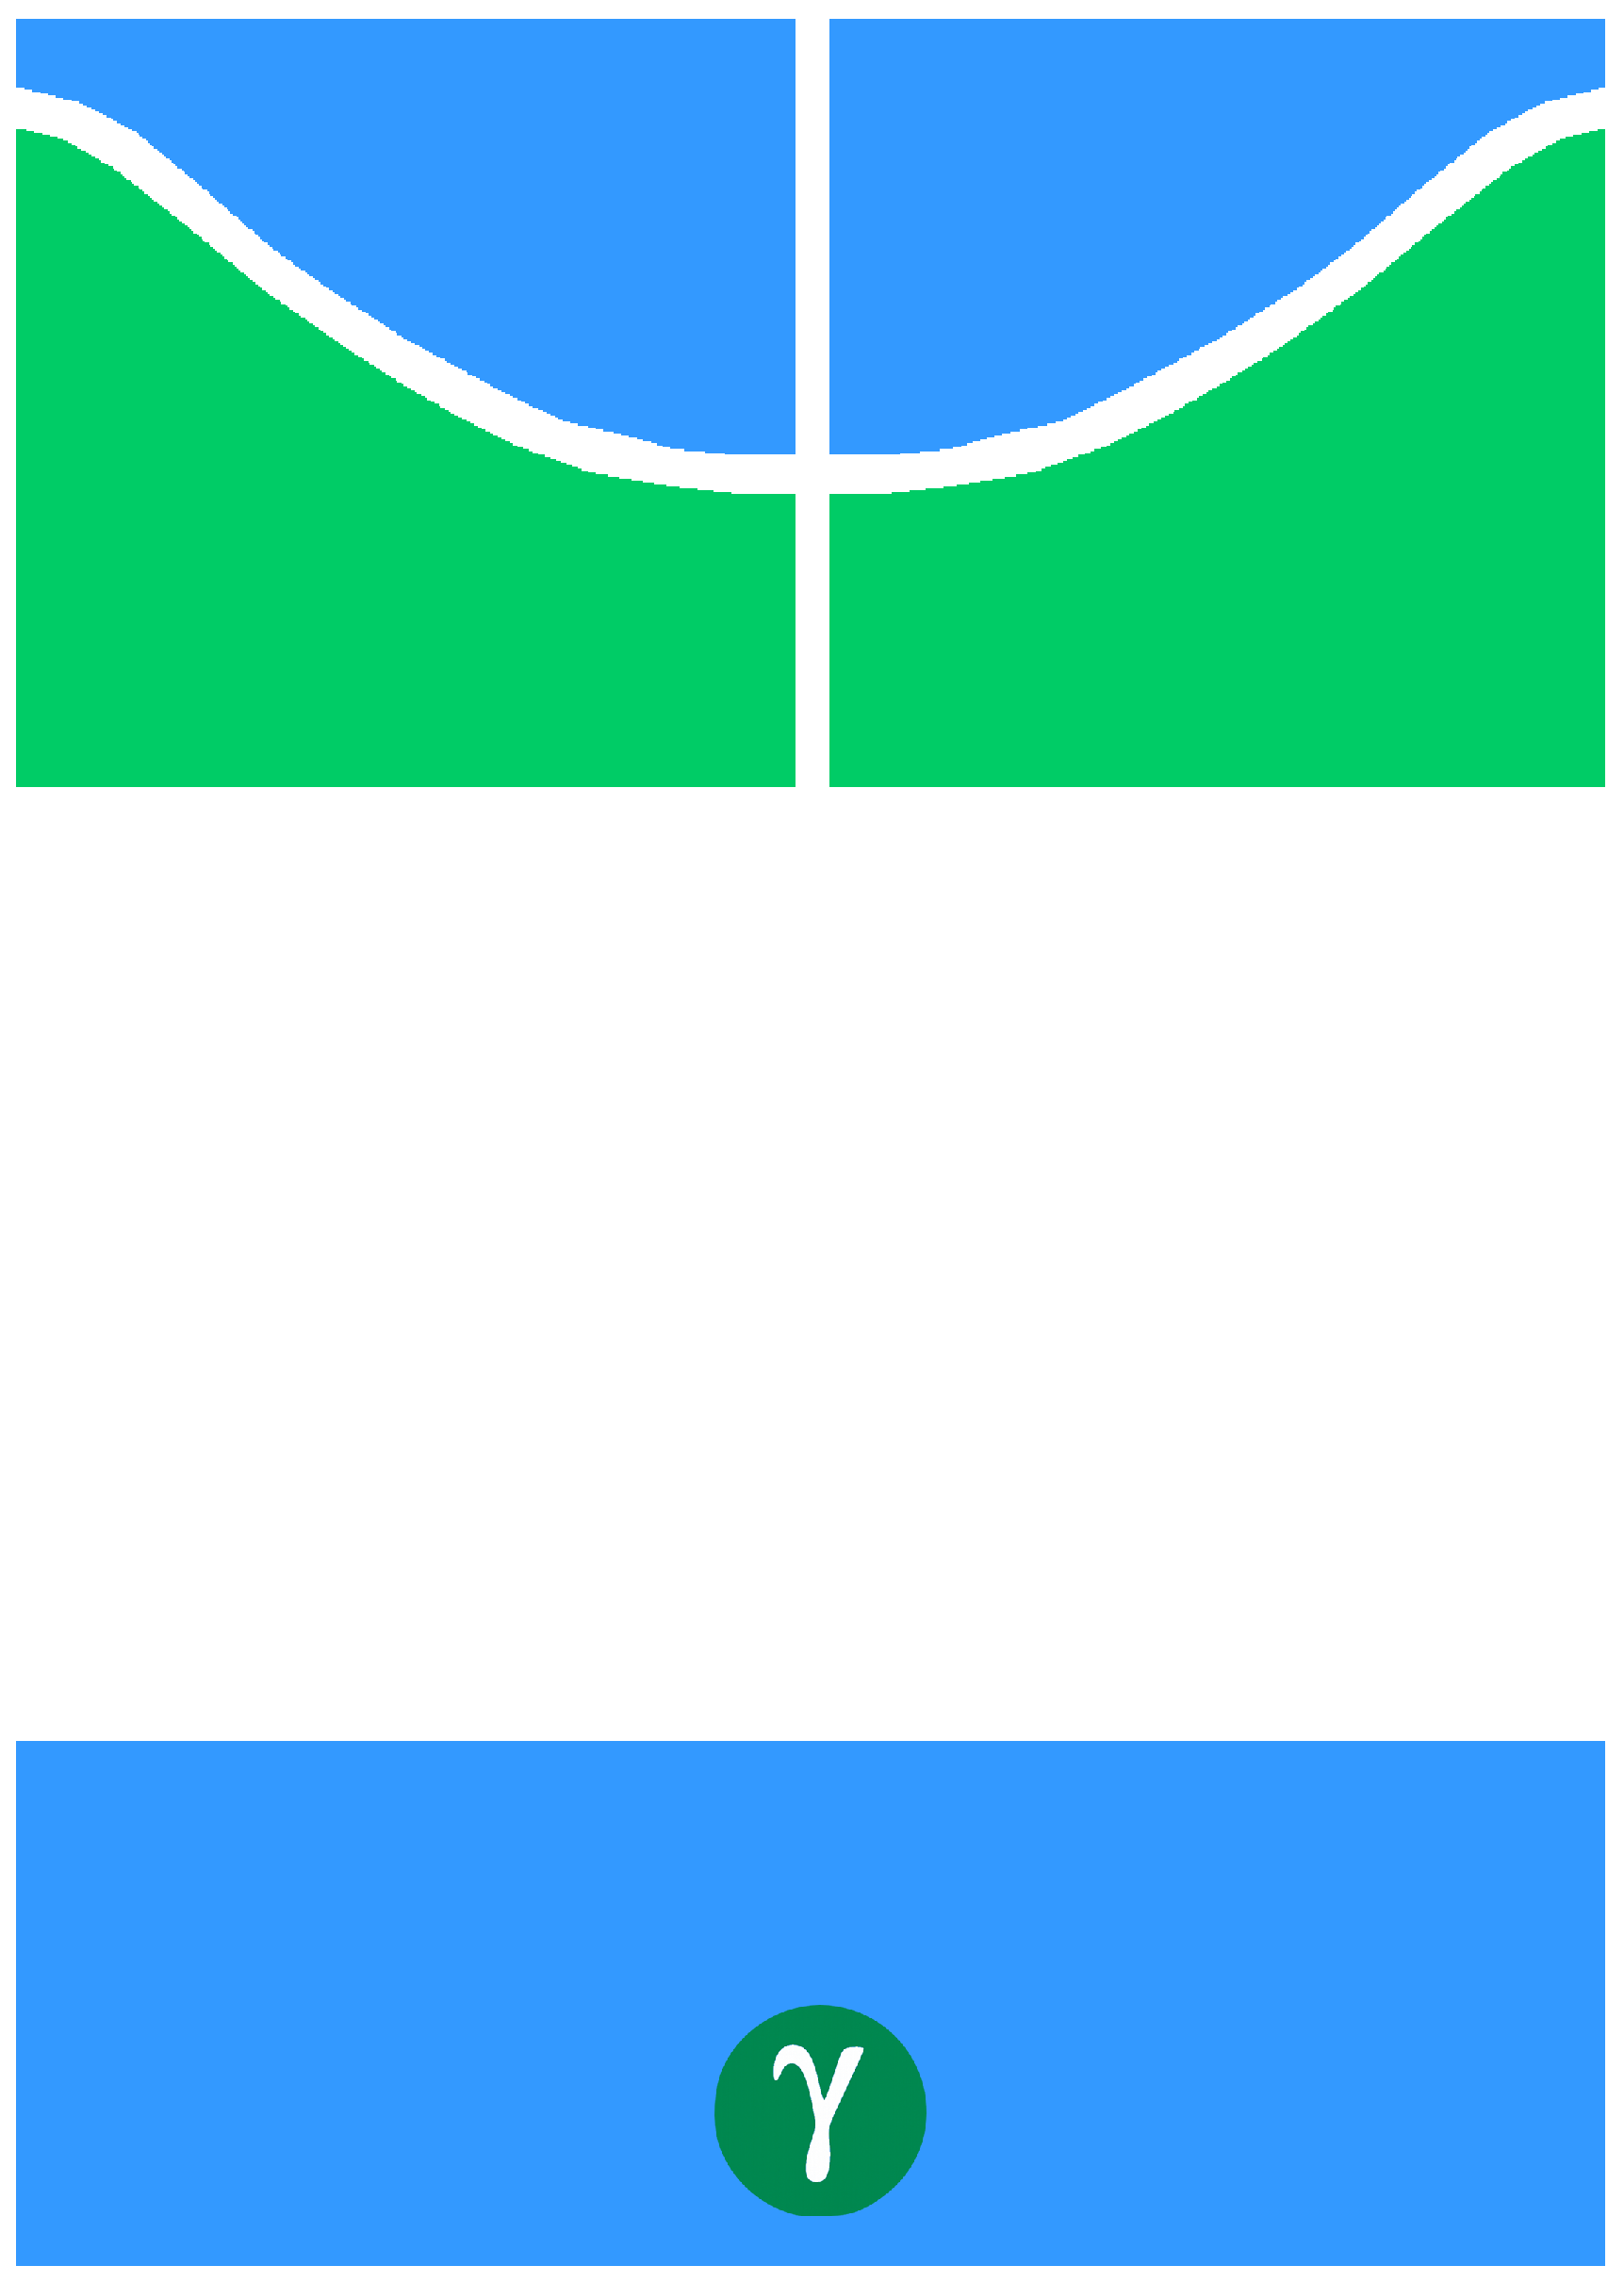
\includegraphics[width=\paperwidth,height=\paperheight,%
				keepaspectratio]{figuras/capa.eps}%
			\vfill
		}
	}
}

\renewcommand{\imprimircapa}{%
  \begin{capa}%
    \center
	\AddToShipoutPicture*{\BackgroundPic}

%	\begin{huge}
%		\textbf{\textsc{Trabalho de Conclusão de Curso}}
%	\end{huge}

    \vspace*{2.7in}
	{\textbf{\large\imprimirinstituicao}}
	\par
	{\textbf{\large\imprimircurso}}

	\vspace{0.5in}

    {\ABNTEXchapterfont\bfseries\LARGE\imprimirtitulo}
    \vspace*{\fill}
    
	\begin{flushright}
    	\textbf{{\large{Autor: \imprimirautor}}}
		\par
    	\textbf{{\large{Orientador: \imprimirorientador}}}
	\end{flushright}
		
    \vspace*{0.2in}
    \textbf{{\large\imprimirlocal}}
    \par
    \textbf{{\large\imprimirdata}}
    
    \vspace*{2.2in}
  \end{capa}
}



% Dados pessoais
\autor{Marcos Roberto Garcia Bahiense Junior}
\curso{SISTEMAS DE INFORMAÇÃO}

% Dados do trabalho
\titulo{CALL CENTER AUTOMATIZADO: INTEGRANDO UM PABX BASEADO EM ASTERIX COM O GSAN}
\data{2015}
\palavraChaveUm{GSAN}
\palavraChaveDois{Asterisk}

% Dados da orientacao
\orientador{Carlos Augusto Mar, M.Sc.}
\coorientador{}

% Dados para a ficha catalográfica
\cdu{02:141:005.6}

% Dados da aprovação do trabalho
\dataDaAprovacao{01 de junho de 2015}
\membroConvidadoUm{Titulação e Nome do Professor Convidado 01}
\membroConvidadoDois{Titulação e Nome do Professor Convidado 02}

\local{Manaus, AM}
\instituicao{%
  Fundação Centro de Análise, Pesquisa e Inovação Tecnológica.
  \par
  Instituto de Ensino Superior FUCAPI
  
}
\tipotrabalho{Trabalho de Conclusão de Curso}
\preambulo{Monografia submetida ao curso de graduação em (\imprimircurso) do Instituto de Ensino Superior FUCAPI – CESF como requisito parcial para obtenção do Título de Bacharel em Sistemas de Informação. Área de concentração: Desenvolvimento e Análise de software.}

\definecolor{blue}{RGB}{41,5,195}
\makeatletter
\hypersetup{
     	%pagebackref=true,
		pdftitle={\@title}, 
		pdfauthor={\@author},
    	pdfsubject={\imprimirpreambulo},
	    pdfcreator={LaTeX with abnTeX2},
		pdfkeywords={abnt}{latex}{abntex}{abntex2}{trabalho acadêmico}, 
		colorlinks=true,       		% false: boxed links; true: colored links
    	linkcolor=blue,          	% color of internal links
    	citecolor=blue,        		% color of links to bibliography
    	filecolor=magenta,      		% color of file links
		urlcolor=blue,
		bookmarksdepth=4
}
\makeatother
\setlength{\parindent}{1.3cm}
\setlength{\parskip}{0.2cm}  
\makeindex


\begin{document}

\frenchspacing 
\imprimircapa
\imprimirfolhaderosto*

\begin{fichacatalografica}
	\vspace*{\fill}					% Posição vertical
	\hrule							% Linha horizontal
	\begin{center}					% Minipage Centralizado
	\begin{minipage}[c]{12.5cm}		% Largura
	
	\imprimirautor
	
	\hspace{0.5cm} \imprimirtitulo  / \imprimirautor. --
	\imprimirlocal, \imprimirdata-
	
	\hspace{0.5cm} \pageref{LastPage} p. : il. (algumas color.) ; 30 cm.\\
	
	\hspace{0.5cm} \imprimirorientadorRotulo~\imprimirorientador\\
	
	\hspace{0.5cm}
	\parbox[t]{\textwidth}{\imprimirtipotrabalho~--~\imprimirinstituicao,
	\imprimirdata.}\\
	
	\hspace{0.5cm}
		1. \imprimirpalavrachaveum.
		2. \imprimirpalavrachavedois.
		I. \imprimirorientador.
		II. PENDENTE.
		III. PENDENTE.
		IV. \imprimirtitulo\\ 			
	
	\hspace{8.75cm} CDU \nomecdu\\
	
	\end{minipage}
	\end{center}
	\hrule
\end{fichacatalografica}

\begin{errata}
Elemento opcional da \citeonline[4.2.1.2]{NBR14724:2011}. \textbf{Caso não 
deseje uma errata, deixar todo este arquivo em branco}. Exemplo:

\vspace{\onelineskip}

FERRIGNO, C. R. A. \textbf{Tratamento de neoplasias ósseas apendiculares com
reimplantação de enxerto ósseo autólogo autoclavado associado ao plasma
rico em plaquetas}: estudo crítico na cirurgia de preservação de membro em
cães. 2011. 128 f. Tese (Livre-Docência) - Faculdade de Medicina Veterinária e
Zootecnia, Universidade de São Paulo, São Paulo, 2011.

\begin{table}[htb]
\center
\footnotesize
\begin{tabular}{|p{1.4cm}|p{1cm}|p{3cm}|p{3cm}|}
  \hline
   \textbf{Folha} & \textbf{Linha}  & \textbf{Onde se lê}  & \textbf{Leia-se}  \\
    \hline
    1 & 10 & auto-conclavo & autoconclavo\\
   \hline
\end{tabular}
\end{table}

\end{errata}

\begin{folhadeaprovacao}

  \begin{center}
    {\ABNTEXchapterfont\large\imprimirautor}

    \vspace*{\fill}\vspace*{\fill}
    {\ABNTEXchapterfont\bfseries\Large\imprimirtitulo}
    \vspace*{\fill}
    
    \hspace{.45\textwidth}
    \begin{minipage}{.5\textwidth}
        \imprimirpreambulo
    \end{minipage}%
    \vspace*{\fill}
   \end{center}
    
   Trabalho aprovado. \imprimirlocal, \imprimirdatadaaprovacao:

   \assinatura{\textbf{\imprimirorientador} \\ Orientador} 
   \assinatura{\textbf{\imprimirmembroconvidadoum} \\ Convidado 1}
   \assinatura{\textbf{\imprimirmembroconvidadodois} \\ Convidado 2}
      
   \begin{center}
    \vspace*{0.5cm}
    {\large\imprimirlocal}
    \par
    {\large\imprimirdata}
    \vspace*{1cm}
  \end{center}
  
\end{folhadeaprovacao}

\begin{dedicatoria}
   \vspace*{\fill}
   \centering
   \noindent
	\textbf{Dedicatória}.

   \textit{
   	 Dedico este trabalho a todos aqueles que vão à luta \\
   	sem medo de perder a batalha, que correm atrás dos  \\
   	seus sonhos e objetivos mesmo que pareça impossível \\
   	alcança-los, a todos aqueles que fazem o bem ao próximo \\
   	sem esperar recompensas e a todos aqueles que mesmo em \\
   	tempos difíceis, acreditam que dias melhores estão por vim.} \vspace*{\fill}
\end{dedicatoria}

\begin{agradecimentos}

\textit{Agradeço primeiramente a Deus, por me privilegiar com a vida, a minha esposa Karoline por ter tido paciência e compreensão durante o período que tive que me dedicar a este trabalho e não me deixar desistir em meio as dificuldades, aos meus familiares por sempre me apoiarem, aos meus amigos por proporcionarem momentos de descontração, meu amigo Wellington que me fez enxergar o potencial deste trabalho e ao meu orientador Carlos Mar que acreditou que seria possível e muito ajudou na concretização deste trabalho.}.

\end{agradecimentos}

\begin{epigrafe}
    \vspace*{\fill}
	\begin{flushright}
		\textit{``Não vos amoldeis às estruturas deste mundo, \\
		mas transformai-vos pela renovação da mente, \\
		a fim de distinguir qual é a vontade de Deus: \\
		o que é bom, o que Lhe é agradável, o que é perfeito.\\
		(Bíblia Sagrada, Romanos 12, 2)}
	\end{flushright}
\end{epigrafe}

\begin{resumo}
Este trabalho apresenta um dos principais sistemas utilizado para gestão de operações comerciais e controle de execução de serviços do setor de Saneamento Básico Brasileiro, o sistema GSAN, com melhorias no que diz respeito ao Atendimento ao Público, resultado da padronização dos atendimentos de primeiro nível e automatização dos atendimentos dos serviços Obter 2ª de Conta, Informar Falta de Água e Solicitar Restabelecimento da Ligação, integrados a uma central de atendimento personalizada através da ferramenta Asterisk, que permite a utilização de voz sobre IP, além do uso convencional da telefonia pública como meio de comunicação com o cliente. Realizado para possibilitar a redução dos custos com atendimento ao cliente e pelo fato das empresas de saneamento serem altamente damandada pela população diariamente. Após o estudo aprofundado dos sistemas envolvidos, foi possível identificar uma forma de integrar as tecnologias de paradígmas diferentes, com a utilização de um agente intermediário responsável pela comunicação via protocolos SOAP e Agi, respectivamente para interligar os sistemas GSAN e Asterisk.  Foram realizados experimentos sobre o produto gerado, após a aplicação dos diversos cenários de testes foi demostrado uma redução de 20,46\% dos registros de atendimentos diários.

 \vspace{\onelineskip}
    
 \noindent
 \textbf{Palavras-chaves}: GSAN. Asterisk. Call Center.
\end{resumo}

\begin{resumo}[Abstract]
 \begin{otherlanguage*}{english}
   This work presents one of the main systems used for managing business operations and execution control services of the Brazilian basic sanitation sector, GSAN system, with improvements with regard to the Public Service as a result of standardization of top-level visits and automation of care services second copy account, Inform Water Lack and Request Restoration of connection, integrated to a central personalized service through Asterisk tool, which allows the use of voice over IP in addition to the conventional use of public telephony as a means communication with the client. Carried out to enable the reduction of customer service costs and because the sanitation companies are highly requested by the population daily. After thorough study of the systems involved, it was possible to identify a way to integrate the different paradigms technologies, using an intermediary agent responsible for communicating via SOAP protocols and AGI respectively to interconnect GSAN and Asterisk systems. Experiments were carried out on the product generated after the implementation of the various scenarios testing was demonstrated a reduction of 20.46\% of daily attendance records.

   \vspace{\onelineskip}
 
   \noindent 
   \textbf{Key-words}: GSAN. Asterisk. Cell Center.
 \end{otherlanguage*}
\end{resumo}

\pdfbookmark[0]{\listfigurename}{lof}
\listoffigures*
\cleardoublepage
\pdfbookmark[0]{\listtablename}{lot}
\listoftables*
\cleardoublepage

\begin{siglas}
	\item[AGI] Asterisk Gateway Interface
	\item[AMI] Asterisk Manager Interface
	\item[CAER] Companhia de Água e Esgotos de Roraima
	\item[CAERN] Companhia de Água e Esgotos do Rio Grande do Norte
	\item[CAJ] Companhia de Águas de Joinville
	\item[COMPESA] Companhia Pernambucana de Saneamento
	\item[CSS] Cascading Style Sheets
	\item[EAR] Enterprise Archive
	\item[EJB] Enterprise Java Beans
	\item[GPL] General Public Lisence
	\item[GSAN] Sistema Integrado de Gestão de Serviços de Saneamento
	\item[IAX] Inter Asterisk eXchange
	\item[IDE] Integrated Development Environment
	\item[IP] Internet Protocol
	\item[JAXB] Java Architecture for XML Binding
	\item[JAX-WS] Java API for XML-BasedWeb Services
	\item[JDK] Java Develop Kit
	\item[JEE] Java Enterprise Edition
	\item[JMS] Java Message Service
	\item[JRE] Java Runtime Environment
	\item[JSP] Java Server Pages
	\item[JVM] Java Virtual Machine
	\item[MC] Ministério das Cidades
	\item[MVC] Model View Controller
	\item[ORM] Object-relational Mapping
	\item[OS] Operating System
	\item[OS] Ordem de serviço
	\item[PA] Posto de Atendimento
	\item[PABX] Private Automatic Branch Exchange
	\item[PMSS] Programa de Modernização do Setor de Saneamento
	\item[QoS] Quality of Service
	\item[RA] Registro de Atendimento
	\item[SGBD] Sistema de Gerenciamento de Banco de Dados
	\item[SIP] Session Initiation Protocol
	\item[SNIS] Sistema Nacional de Informações do Setor de Saneamento
	\item[SNSA] Secretaria Nacional de Saneamento Ambiental
	\item[SOAP] Simple Object Access Protocol
	\item[URA] Unidade de Resposta Audível
	\item[URL] Uniform Resource Locator
	\item[VoIP] Voice over Internet Protocol
	\item[WAV] WAVE
	\item[WEB] World Wide Web
	\item[WSDL] Web Services Description Language
	\item[XML] eXtensible Markup Language.
\end{siglas}

\begin{simbolos}
  \item[$ \Gamma $] Letra grega Gama
  \item[$ \Lambda $] Lambda
  \item[$ \zeta $] Letra grega minúscula zeta
  \item[$ \in $] Pertence
\end{simbolos}

\pdfbookmark[0]{\contentsname}{toc}
\tableofcontents*
\cleardoublepage


\textual
% INICIO - INTRODU��O 
\chapter[Introdução]{INTRODUÇÃO}
%\addcontentsline{toc}{chapter}{Introdução}

A Secretaria Nacional de Saneamento Ambiental (SNSA) que integra o Ministério das Cidades (MC) visando elevar o nível de desempenho e eficiência das empresas de abastecimento de água e coleta de esgoto teve a iniciativa de promover o desenvolvimento de um software que pudesse atender as necessidades básicas do setor de saneamento de um modo geral. \\[0.2cm]

Por meio do Programa de Modernização do Setor de Saneamento \cite{PMSS:2014} efetuou a contratação de uma empresa de tecnologia da informação brasileira para executar o projeto concebido.  Nesse cenário, surge então o sistema GSAN\footnote{GSAN - Sistema Integrado de Gestão de Serviços de Saneamento.} que se trata de um sistema desenvolvido com tecnologias de software livre, para a gerência de operações comerciais e de controle da execução de serviços internos das companhias de saneamento, o software atualmente encontra-se disponível gratuitamente no portal do software público brasileiro \cite{PORTAL:2014}. 

Mesmo com a modernização do setor de saneamento através do sistema GSAN que atualmente está implantado em 10 companhias estaduais das quais 4 estão em processo de migração \cite{PMSS:2014}, ainda há grandes desafios a serem superados e um deles será abordado neste trabalho.

O Atendimento ao público trata-se de uma das frentes que as empresas de saneamento necessitam disponibilizar aos seus clientes. Muitas das vezes o valor envolvido em manter disponível uma infraestrutura que atenda a necessidade da empresa, com equipes de \textit{Call Center} ou mesmo com atendimento presencial, podem gerar custos astronômicos dependendo da quantidade e qualidade da mão de obra contratada, aquisição de licenças para soluções proprietárias entre outros fatores que podem contribuir para variação do valor. 

Atualmente o uso de software \textit{Open Source} nas empresas tem se tornado bastante comum \cite{MEIRELLES2014}, com intuito de apoiar o negócio, como é o caso do software Asterisk que implementa facilidades no uso de tecnologias como PABX\footnote{PABX - \textit{Private Automatic Branch Exchange.}}  tanto para linhas telefônicas convencionais como também por VoIP\footnote{VoIP - \textit{Voice over Internet Protocol}} que utiliza a transmissão de voz sobre um rede IP\footnote{IP - \textit{Internet Protocol}} com padrão de qualidade de serviço (QoS), permitindo a utilização de URA (Unidade de Resposta Audível) \cite{VIEIRA:2007} como linha de frente no atendimento ao cliente.



\section*{Problema}

Atualmente o GSAN, atende grande parte das companhias de saneamento brasileiras, como é o caso de companhias como por exemplo CAERN\footnote{CAERN - Companhia de Água e Esgotos do Rio Grande do Norte}, CAER\footnote{CAER - Companhia de Água e Esgotos de Roraima}, COMPESA\footnote{COMPESA - Companhia Pernambucana de Saneamento}, MANAUS AMBIENTAL entre outras citadas no seguinte referencial teórico \ref{key:GSAN-TEORIA}.

Essas empresas fazem uso do sistema para gerenciar as suas informações operacionais e gerenciais, que de certa forma atende as demandas internas. Entretanto, no aspecto do atendimento ao público, existem lacunas que ainda precisam ser atendidas de forma plena, principalmente por se tratarem de organizações altamente demandadas pela população, sendo responsáveis por atender diversos tipos de clientes que variam desde pequenos vilarejos até grandes metrópoles.

A falta de padronização nos atendimentos, o grande fluxo de transferência entre ramais e a variação nos tempos de atendimentos são muito comuns, pelo fato de todo atendimento de Primeiro Nível\footnote{Atendimento de Primeiro Nível Refere-se a recepção inicial de todo atendimento.} normalmente ser realizado por pessoas ou PA\footnote{PA - Posto de Atendimento}, ou seja, são recursos caros. Normalmente os atendentes respondem por um determinado setor da empresa, encarregado em solucionar tipos específicos de problemas, possibilitando muita das vezes a realização de transferência para outros ramais até que o cliente consiga concluir uma solicitação, o que pode gerar desconforto e insatisfação com os serviços de atendimento.
	
Existe uma grande dificuldade das empresas de saneamento, em disponibilizar uma estrutura de \textit{Call Center} que atenda as expectativas dos clientes.

A dificuldade em manter um \textit{feedback} rápido com o cliente, a falta de canais de comunicação flexíveis que permitam uma disponibilidade maior inclusive fora do horário comercial, a ineficiência na triagem dos atendimentos, são questões rotineiras enfrentadas no cotidiano das empresas de saneamento.

\section*{Objetivo}
%\addcontentsline{toc}{section}{Objetivo}
% Adiciona item no sumário

A finalidade deste trabalho propõe atender ao objetivo geral e aos objetivos específicos descritos a seguir.

\subsection*{Objetivo Geral}

Desenvolver uma integração do sistema GSAN (Sistema Integrado de Gestão de Serviços de Saneamento) com uma ferramenta de PABX (\textit{Private Automatic Branch Exchange}) que permita o atendimento automático de chamadas telefônicas via tecnologia VoIP destinados à obter 2ª via de conta, informar falta de água e solicitar restabelecimento da ligação de água.

\subsection*{Objetivo Específico}
Para alcance deste objetivo, fazem necessários os seguintes passos:
\begin{itemize}
	\item Implementar a integração entre o sistema GSAN com uma ferramenta de PABX.
	\item Elaborar cenários de teste para os serviços obter 2ª via de conta, informar falta de água e solicitar restabelecimento da ligação de água.
	\item Desenvolver uma suíte de testes automatizados com foco na integração dos sistemas. 
	\item Contribuir com a comunidade do sistema GSAN, disponibilizando a nova funcionalidade desenvolvida.
\end{itemize}
\section{Justificativa}
A integração entre sistema GSAN com uma ferramenta de PABX será um experimento de cunho prático, realizado para atender a uma grande demanda do setor de saneamento brasileiro, que atualmente sofre com a dificuldade em fornecer uma comunicação efetiva e eficiente através de seu sistema de informação principal que atenda as expectativas dos clientes.
Com base nas informações disponibilizadas, no Relatório de Análise Regulatória da Companhia de Águas de Joinville (CAJ) (AMAE, 2015) situada em no estado de Santa Catarina, divulgado em 2014, demonstra a ineficiência enfrentada pelo setor de saneamento no que diz respeito ao Atendimento ao Público, a companhia considerada universalizada por atender mais 99\% da população urbana com abastecimento de água, somando um total de aproximadamente 508.097 habitantes no município, atualmente enfrenta um número acentuado de reclamações, conforme demonstrado na figura 1 abaixo:
 

\begin{figure}[!htb]
	\centering
	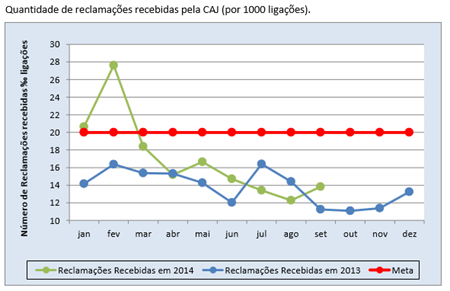
\includegraphics{figuras/LigacoesReclamacoes.png}
	\caption{Gráfico da Quantidade de Reclamações Mensais da CAJ}	
	Fonte - Companhia Águas de Joinville, 2014
\end{figure}


 Em 2013 o indicador de Número de Reclamações apresentou uma média anual de 13,78 reclamações/mil ligações de água, com uma quantidade notória de reclamações diárias se tornar custoso atender a todas solicitações individualmente utilizando somente atendentes sem que haja otimizações nos atendimentos, refletindo na média anual do tempo de espera das ligações para o \textit{Call Center} da companhia que no ano de 2013 que apresentou o tempo de 75,2 segundos por atendimento, deixando evidente o quão necessário se faz adotar medidas de melhorias nos sistemas de \textit{Call Center}. Conforme informações disponíveis no Sistema Nacional de Informações do Setor de Saneamento (SNIS) (SNIS, 2014), especificamente a Região Norte do país possui um dos piores índices de perda de faturamento do país, consequentemente isso gera lucros menores e ineficiência na ampliação do acesso à população aos serviços de saneamento, dificultando ainda mais investimentos por parte das companhias em tecnologias renovadores para o setor de saneamento. Visando propor soluções viáveis que possam agregar valor à empresa sem acarretar em custos elevados, utilizando de soluções em software \textit{Open Source} com tecnologias compatíveis, será possível tornar o próprio sistema principal de uma empresa de saneamento o GSAN, capaz de suprir através dos recursos da ferramenta Asterisk a necessidade em disponibilizar de forma prática e padronizada o acesso a informações geradas e mantidas pela empresa, consequentemente possibilidade de redução de custo com a utilização de uma unidade de resposta audível para realizar o atendimento de primeiro nível. Propiciando ao cliente final um melhor e mais efetivo relacionamento com a empresa prestadora de serviços.


\section{Aspectos de Inovação}
O trabalho de pesquisa e desenvolvimento se trata de uma integração entre software totalmente distintos, com tecnologia Open Source, onde juntos seram capazes de atender à uma demanda existente no setor de saneamento brasileiro relacionado ao contexto de Atendimento ao Público. Com a integração entre o sistema GSAN com o software Asterisk, será possível transferir os atendimentos destinado a central de atendimento, para uma Unidade de Resposta Audível (URA), executando a triagem das solicitações de forma padronizada e para solicitações referentes aos tipos de serviços Obter 2ª via de Conta, Informar Falta de Àgua e Solicitar Restabelecimento de Ligação, será possível realizar de forma automatizada o atendimento, sem que haja intervenção humana durante o processo. 
Não há oficialmente uma versão publicada na comunidade do sistema GSAN capaz de atender esta demanda de forma igual ou superior, inovando em propor uma solução viável e eficiente de baixo custo, para possibilitando a melhoria no atendimento ao cliente, se destacando em permitir que o cliente possa realizar suas solicitações em qualquer horário do dia ou noite, sem ter que se locomover a empresa e acessar informações de débitos pendentes de forma rápida e padronizada.

\section*{Trabalhos Relacionados}
Este trabalho de pesquisa e desenvolvimento se assemelha ao trabalho descrito por Guilherme \cite{VIEIRA:2007}, que também utilizou recursos do programa Asterisk para desenvolver uma Sistema de criação de planos de discagem de forma prática explanando aspectos da ferramenta e expondo as dificuldades encontradas, apesar de ambos utilizarem dos diversos recursos do Asterisk, há divergência no objetivo onde este se destaca o fato de realizar uma integração com outro software, visando solucionar uma demanda do setor de Saneamento.

No trabalho desenvolvido por Jilcimaico \cite{DARU:2008}, aborda com clareza a utilização da distribuição Disc-OS como interface WEB do Asterisk, além de descrever os principais conceitos envolvidos na utilização do software, demonstra os procedimentos necessários para realizar a instalação da ferramenta e configuração dos recursos essências para um \textit{Call Center}, assemelhando-se este ao fato de também utilizar a distribuição Disc-OS que propõe uma interface WEB para a configuração do Asterisk.

O trabalho desenvolvimento por Humberto \cite{CAMPOS:2007}, utilizou os principais recursos do software Asterisk para realizar uma integração com um sistema externo que calcula os valores de cada ligação realizada, módulo chamado de “tarifador” além de exibir os valores em um hardware próprio, tal integração utilizou como referência tabelas em banco de dados para reconhecer eventos ocorridos e ações a serem tomadas, assemelhando-se a este trabalho pelo fato de utilizar recursos do Asterisk para disparar ações de sistemas externos, no entanto a forma de integração retratada acima se diferencia da forma adotada neste trabalho, que utiliza a interface AGI disponibilizada para comunicação com sistemas externos, o próprio Asterisk irá disparar ações a serem realizadas por meio de um \textit{Middleware} que implementa esta interface de comunicação.

Atualmente a empresa de saneamento Companhia Pernambucana de Saneamento \cite{COMPESA:URA} disponibilizou aos seus clientes o atendimento eletrônico por meio de URA, possibilitando a empresa realizar o atendimento destinado a central de atendimento, ou seja, o atendimento de primeiro nível, de forma automática e padronizada, propiciando também os direcionamentos entre ramais reais da empresa agilizando o atendimento e potencializando uma disponibilidade de 24 horas por 7 dias, com as informações à disposição dos clientes remotamente, porém a empresa não divulgou detalhes técnicos ou artefatos produzidos para realizar tal integração ou customização.
Para auxílio na elaboração deste trabalho de pesquisa se fez de grande valia os detalhes apontados sobre o \textit{software} Asterisk, principalmente a conceituação e protocolos disponibilizados para comunicação com sistemas externos, contidos no próprio \textit{website} da \textit{Digium \footnote{Disponível em: \url{http://www.digium.com/}}}. 

\section*{Método de Investigação}
A metodologia utilizada para realização do presente trabalho foi dívida da seguinte forma:
\begin{itemize}
	\item Pesquisa bibliográfica para obter o embasamento teórico sobre funcionamento dos sistemas envolvidos
	\item Identificação de uma possível forma de integração entre ambos;
	\item Desenvolvimento da integração entre os sistemas.
	\item Desenvolvimento de uma suíte de testes automatizados.
	\item Experimentação utilizando a suíte de testes automatizados
\end{itemize}

\section*{Estruturação da Monografia}
	
Após este capítulo introdutório, que basicamente visa contextualizar e caracterizar o tema de pesquisa, o trabalho realizado foi dividido em sete capítulos, conforme descrito abaixo:
\begin{description}
	\item \textbf{Capítulo 2} – Fundamentação Teórica – Este capítulo tem como objetivo abordar alguns dos conceitos do saneamento brasileiro e como o sistema GSAN está construído para atendê-lo, quais os módulos que compõem o sistema e detalhar a arquitetura do sistema, assim como expor os conceitos que envolvem o software Asterisk.
	\item \textbf{Capítulo 3 } – Revisão Bibliográfica – Será apresentado os principais conceitos utilizados como base no desenvolvimento deste trabalho.
	\item \textbf{Capítulo  4} – Processo de Integração – Trata-se da implementação realizada para integração entre os sistemas, apresentando as principais etapas para elaboração da comunicação entre os sistemas.
	\item \textbf{Capítulo  5} – Experimentação Utilizando a Suíte de testes Automatizados – Tem como característica a preparação do ambiente de teste, o planejamento e execução das experimentações utilizando a suíte de testes automatizados para validar a integração entre o sistema GSAN com o \textit{software} Asterisk.
	\item \textbf{Capítulo 6} – Conclusão – Neste capítulo, apresenta-se as conclusões que foram obtidas a partir deste trabalho.
	\item \textbf{Capítulo 7} – Considerações Finais e Trabalhos Futuros – Finalmente, no sétimo capítulo, apresentam-se recomendações para trabalhos futuros, reunindo os comentários finais deste trabalho de pesquisa.	
\end{description}
	

\section*{Cronograma}
A seguir será apresentado o cronograma com o planejamento mensal do início e termino das atividades previstas para conclusão do trabalho de pesquisa.

\begin{table}[htb]
	\center
	\footnotesize
	\begin{tabular}{|p{5cm}|p{0.8cm}|p{0.8cm}|p{0.8cm}|p{0.8cm}|p{0.8cm}|p{0.8cm}|p{0.8cm}|p{0.8cm}|}
		\hline
		\centering
		\textbf{Atividade} & \textbf{Jun} & \textbf{Jul} & \textbf{Ago} & \textbf{Set} & \textbf{Out} & \textbf{Nov} & \textbf{Dez}\\
		\hline
		Pesquisa bibliográfica. 			& \textbullet & \textbullet & - & - & - & - & - \\
		\hline
		Identificar formas de integração.	& - & \textbullet & \textbullet & - & - & - & - \\
		\hline
		Implementar a integração. 			& - & - & \textbullet & \textbullet & \textbullet & - & -  \\
		\hline
		Realizar experimentos. 				& - & - & - & - & \textbullet & \textbullet & - \\
		\hline
		Escrita da monografia. 				& \textbullet & \textbullet & \textbullet & \textbullet & \textbullet & \textbullet & \textbullet \\
		\hline
		Apresentação da monografia. 		& - & - & - & - & - & - & \textbullet \\		
		\hline
	\end{tabular}
\end{table}



% FUNDAMENTACAO
\chapter[Fundamentação Teórica]{\textbf{F}undamentação \textbf{T}eórica}
%\addcontentsline{toc}{chapter}{Fundamentação Teórica}

\textit{Neste capítulo será apresentado o sistema GSAN e software Asterisk, com a intenção de familiarizar o leitor com as notações que serão amplamente utilizadas no decorrer do trabalho.}


\section{GSAN}
O sistema de código aberto GSAN\label{key:GSAN-TEORIA} (Sistema Integrado de Gestão de Serviços de Saneamento) desenvolvido inicialmente pela empresa IPAD (Instituto de Planejamento e Apoio ao Desenvolvimento Tecnológico e Científico) em 2005 por meio do Programa de Modernização do Ministério da Cidades, atualmente mantido e disponibilizado pelo Portal de Software Livre Brasileiro, sendo constantemente melhorado e aperfeiçoado pelos prestadores de serviços e interessados. 

Propõem-se em atender as principais demandas de gestão de operações comerciais e controle de execução de serviços nas companhias de saneamento do Brasil, que atualmente utilizam o sistema em grande escala, conforme exposto a seguir pela figura \ref{figura:implantacaoSistemaGSAN}:


\begin{figure}[H]
	\centering
	\caption{Implantações do Sistema GSAN}	
	\label{figura:implantacaoSistemaGSAN}
	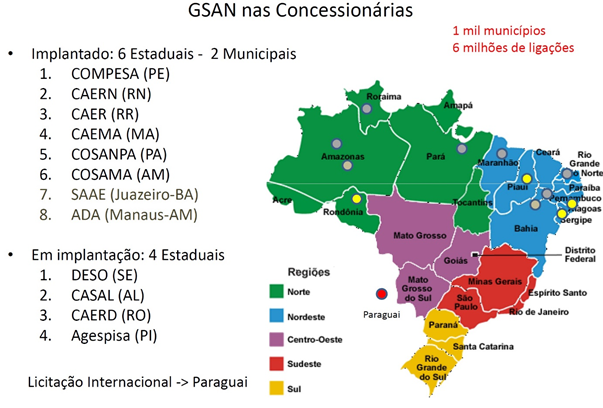
\includegraphics{figuras/implantacaoGSAN.png}
	\legend {\fontsize{10}{12}\selectfont {Fonte: \citeonline{PORTAL:2014}}.}
\end{figure}


Conforme demonstrado acima o sistema está em funcionamento em aproximadamente 1 mil municípios brasileiros, concentrado principalmente na região Norte e Nordeste do Brasil.
Atualmente o sistema está preparado para atender companhias de pequeno e médio porte, provendo soluções flexíveis através de parametrizações em tabelas de banco de dados, adequando-se a realidades distintas e tornando-se referência em software para o setor de saneamento básico brasileiro. 

\subsection{GSAN Conceitos}

O sistema em sua concepção foi dividido nos seguintes módulos descritos abaixo:
\begin{itemize}
\item \textbf{Atendimento ao Público}: Responsável principalmente em fornecer acesso rápido as informações dos clientes/imóveis e possibilita o registro dos atendimentos realizados.
\item \textbf{Cadastro}: Responsável em permitir a inserção, alteração e exclusão das entidades básicas só sistema.
\item \textbf{Micromedição}: Aborda as regras de consistência e análise de leitura e consumo, provendo meios para verificar o comportamento do consumo de água do imóvel.
\item \textbf{Faturamento}: Responsável principalmente em realizar o cálculo para precificar o consumo e gerar/emitir as faturas.
\item \textbf{Arrecadação}: Disponibiliza meios para efetuar a baixa de débitos dentre outras rotinas dessa natureza.
\item \textbf{Segurança}: Possibilita a gestão sobre as permissões de usuários/funcionários.
\item \textbf{Cobrança}: Fornece meios de emitir formas de cobranças personalizadas.
\item \textbf{Contabilização}: Realiza a contabilidade e possibilita integrações para sistemas externos.
\end{itemize}

Alguns dos conceitos de saneamento serão abordados neste trabalho, portanto faz-se necessário conhecer e entender como o sistema GSAN aborda essas questões.

O imóvel no sistema deve possuir relação com os seguintes itens (Tabela \ref{tabela:atributosImovel}):
\begin{table}[H]
	\center
	\footnotesize
	\caption{Principais Atributos do Imóvel}
	\label{tabela:atributosImovel}
	\begin{tabular}{|p{3cm}|p{7cm}|p{2.5cm}|} \hline
		\textbf{Atributo} 	& \textbf{Descrição}						& \textbf{Obrigatório}  \\ \hline
		Localidade 			& Um conjunto populacional					& Sim \\	\hline
		Setor Comercial 	& Conjunto de quadras, semelhante ao bairro & Sim \\ 	\hline
		Quadra 				& Denominado normalmente de "quarteirão" 	& Sim \\ 	\hline			
		Lote 				&  Uma subdivisão da Quadra 				& Sim \\ 	\hline
		Sub-Lote 			&  Uma subdivisão da Lote 					& Sim \\ 	\hline
	\end{tabular}
	\legend {\fontsize{10}{12}\selectfont {Fonte: Autoria Própria}.}
\end{table}


Tais relacionamentos são necessários para constituir a matrícula do imóvel, que forma um código único e representa a localização exata do imóvel.\\
\textbf{Matrícula:} [ Localidade ].[ Setor Comercial ].[ Quadra ].[ Lote ].[ Sub-Lote ]  \\
\textit{Ex: 001.015.080.0120.001}

O imóvel pode conter uma Ligação seja ela de Água, Poço e Esgoto, após o cliente realizar o cadastro do imóvel e solicitar a ligação, normalmente quando o imóvel obtém uma Ligação de Água ou Poço, é cobrado uma taxa mensal referente ao Esgoto variando em muito dos casos de 80\% a 100\% do valor a ser cobrado pelo consumo de água. Existem as possíveis situações para a Ligação do imóvel:
\begin{itemize}
	\item \textbf{Ligado}: Imóvel está conectado à rede de distribuição de água.
	\item \textbf{Potencial}: Imóvel está localizado fora do alcance da rede de distribuição de água.
	\item \textbf{Factível}: Imóvel está localizado dentro do alcance da rede de distribuição de água, mas que nunca esteve conectado a ela.
	\item \textbf{Cortado}: Imóvel que possui um dispositivo de vedação do fluxo de água no intuito de interromper o abastecimento.
	\item \textbf{Suprimido}: Imóvel que teve o ramal de água retirado para a interrupção definitiva do abastecimento de água.	
\end{itemize}

O relacionamento entre Clientes e Imóveis no sistema pode ocorrer das seguintes formas:
\begin{itemize}
	\item \textbf{USUÁRIO} – Pessoa que reside no imóvel.
	\item \textbf{PROPRIETÁRIO} – Pessoa que possui a propriedade do bem de direito.
	\item \textbf{RESPONSÁVEL} – Pessoa responsável pelo pagamento de débitos do imóvel.	
\end{itemize}

As solicitações realizadas pelos clientes aos atendentes são denominadas Registros de Atendimentos pelo sistema, comumente chamada de RA, para cada tipo de solicitação seja ela Solicitar Ligação, Solicitar Corte, Informar Falta de Água entre outras, o sistema possui tipos de serviços que devem ser realizados para atender à solicitação, a execução destes serviços é representado por uma  entidade denominada Ordem de Serviço, comumente chamada de OS, o sistema permite que seja configurada a criação de OS automáticas para determinadas solicitações, tornando menos burocrático a formalização das reclamações recebidas.


\subsection{GSAN Arquitetura}
	
O Sistema GSAN foi desenvolvido fundamentalmente utilizando a plataforma JEE\footnote{JEE - \textit{Java Enterprise Edition}}, propriedade da \textit{Oracle Corporation}, em sua versão 5, na época a mais recente. Utiliza os principais serviços e tecnologias oferecidos pela plataforma, como por exemplo, EJB\footnote{EJB - \textit{Enterprise Java Beans}}, JMS\footnote{JMS - \textit{Java Message Service}} e JSP\footnote{JSP - \textit{Java Server Pages}} 2.1.
O GSAN possui uma arquitetura que implementa diversos padrões de projeto, visando facilitar a manutenibilidade e manter a organização dos componentes, segue abaixo o diagrama de componentes conforme a figura \ref{figura:arquiteturaDetalhada}:

\begin{figure}[H]
	\centering
	\caption{Arquitetura Detalhada do Sistema GSAN}	
	\label{figura:arquiteturaDetalhada}
	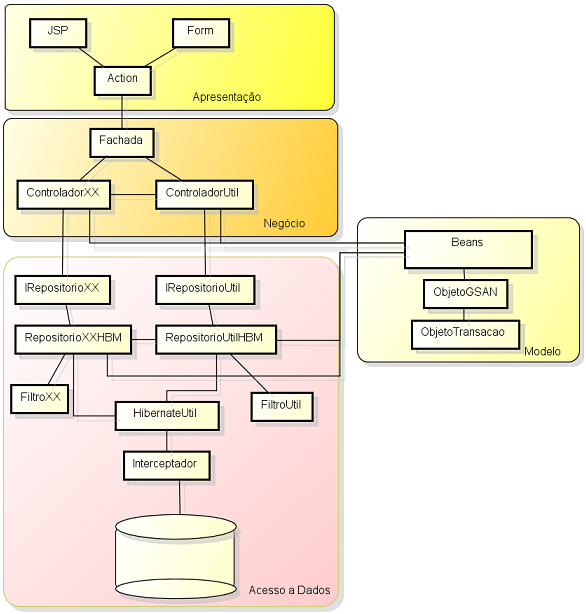
\includegraphics{figuras/gsanArquiteturaMenor.png}
	\legend {\fontsize{10}{12}\selectfont {Fonte: Autoria Própria}.}
\end{figure}

	
A camada de apresentação utiliza recurso nativo da plataforma JEE para Web, sendo a JSP para construção dos layouts e páginas a serem exibidas, juntamente com o \textit{framework} Apache Struts versão 1.2 atuando como controlador das requisições, além de Javascript e CSS para tratar o comportamento e aparência das páginas.
A fachada é um ponto de comunicação entre as camadas de apresentação e a camada de negócio e implementa o padrão de projeto \textit{Singleton}\footnote{\textit{Singleton} refere-se ao Padrão de Projeto que garante a existência de somente uma instância de determinada classe.}. 
A principal função da fachada é centralizar todas as chamadas de métodos da camada de negócio para que outras aplicações ou outras camadas superiores possam utilizar seus serviços.
As Classes de Controladores EJB são responsáveis por garantir toda a regra de negócio do sistema, elas são implementadas utilizando a especificação do \textit{Enterprise Java Beans} versão 2.1.
As classes de Repositório são classes da aplicação que utilizam o padrão de projeto \textit{Singleton}, a responsabilidade desta classe consiste em assegurar que todos os métodos de persistência ou serviço de consulta com o banco de dados.

O sistema GSAN foi projetado para ser independente da solução de Banco de Dados utilizada, acoplado ao \textit{framework} Hibernate que trata da persistência Objeto/Relacional (ORM), possibilita o isolamento da camada de Persistência.

A aplicação dos Padrões de Projetos renomados, tornar o código mais organizado e entendível, facilitando futuras manutenções, a utilização do padrão MVC\footnote{MVC - \textit{Model View Controller}} como estrutura arquitetural faz com que exista isolamento entre as camadas de Modelo, Visualização e Controle da aplicação, tornando a organização de pacotes bem estruturada.
	
	
\subsection{GSAN Configuração}
A configuração do ambiente de desenvolvimento se trata de um passo fundamental para execução deste trabalho prático. Primeiramente será preciso obter a versão do sistema que se encontra disponível no site do Portal do Software Livre, que atualmente disponibiliza o código fonte do sistema GSAN e demais arquivos de configuração do ambiente, no \textit{github}\footnote{Disponível em \url{http://www.github.com}} para a comunidade de desenvolvedores e interessados. 

Com o código fonte em mãos é necessário o auxílio de uma IDE\footnote{IDE - \textit{Integrated Development Environment}} de desenvolvimento para realizar a manutenção e construção dos novos serviços, foi utilizado neste trabalho a IDE Eclipse Juno para realizar esta tarefa, o processo de configuração da IDE pode ser visto descrito nos anexos deste trabalho.

O processo de empacotamento para geração do EAR (\textit{Enterprise Archive}) para disponibilização, utiliza a ferramenta Apache Ant versão 1.6.2, normalmente a versão disponibilizada pela comunidade possui \textit{script} de \textit{build}\footnote{\textit{Scripts} de \textit{build} refere-se a instruções para realizar o empacotamento da aplicação.} para serem executados, no entanto é preciso configurar os locais adequados para geração do pacote, conforme segue o exemplo abaixo na figura \ref{figura:configuracaoScriptBuild}:

\begin{figure}[H]
	\centering
	\caption{Exemplo de configuração do \textit{script} build}
	\label{figura:configuracaoScriptBuild}	
	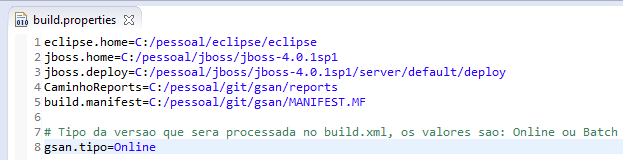
\includegraphics{figuras/build_properties.png}
	\legend {\fontsize{10}{12}\selectfont {Fonte: Autoria Própria}.}
\end{figure}
	
A execução do \textit{script} pode ser realizada dentro da IDE executando o seguinte procedimento, após localizar o arquivo \textit{build.xml} dentro na raiz do projeto, ao clicar com o botão esquerdo e selecionar a opção \textit{Run as > Ant Build}, será acionado a execução da instrução \textit{make} padrão do \textit{script}, para construção do pacote a ser disponibilizado, conforme visto na figura \ref{figura:execucaoScriptBuild}:	
		
\begin{figure}[H]
	\centering
	\caption{Execução do \textit{script} de build}
	\label{figura:execucaoScriptBuild}
	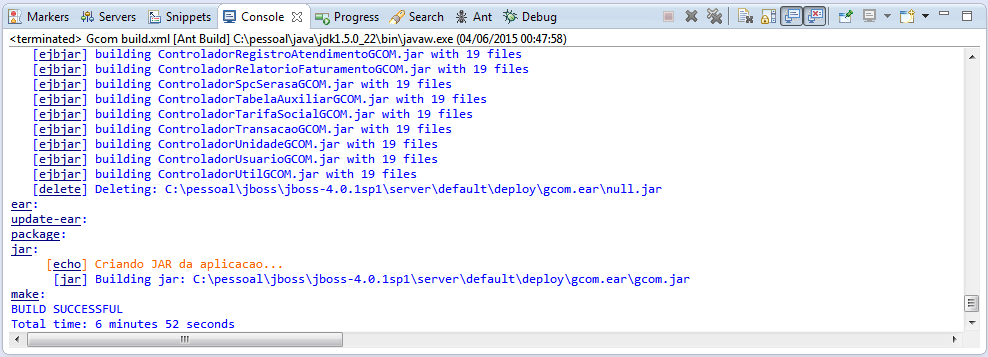
\includegraphics{figuras/build_ant.png}
	\legend {\fontsize{10}{12}\selectfont {Fonte: Autoria Própria}.}
\end{figure}

Para executar a aplicação faz-se necessário a utilização de um servidor de aplicação que implemente as principais interfaces de serviços da plataforma JEE que serão consumidos pela aplicação, neste trabalho foi utilizado o projeto \textit{Open Source Jboss Community} na versão 4.0.1, compatível com as tecnologias utilizadas no GSAN, a configuração deste Servidor de Aplicação Web pode ser consultado nos anexos deste trabalho.
Para executar o sistema GSAN, utilizando o terminal de comando do sistema operacional (\textit{Command Prompt}) basta digitar run e pressionar a tecla Enter será iniciado o servidor de aplicação e executará o sistema GSAN, visto na figura \ref{figura:execucaoSistemaGSAN}:


\begin{figure}[H]
	\centering
	\caption{Executando o sistema GSAN}	
	\label{figura:execucaoSistemaGSAN}
	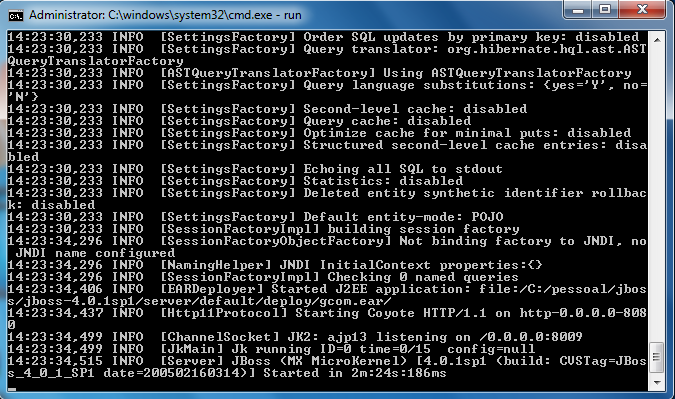
\includegraphics{figuras/executando_jboss.png}	
	\legend {\fontsize{10}{12}\selectfont {Fonte: Autoria Própria}.}
\end{figure}


A solução adotada para banco de dados neste trabalho será o PostgreSQL na versão 9.3.4 e PgAdmin versão 1.18.1 como SGBD (Sistema de Gerenciamento de Banco de Dados), no próprio site existe o guia de instalação para desenvolvedores tornando esse passo bem intuitivo.

Na versão do sistema GSAN disponibilizada para a comunidade, existe um diretório chamado \textbf{\textit{migrations}} que contém os \textit{scripts} de banco de dados necessários para criação das tabelas principais que o sistema exige para funcionar corretamente, e também disponibiliza todas instruções necessárias para a configuração dos datasources comercial e gerencial que serão utilizados no sistema GSAN.
Para acessar o sistema em execução, basta digitar o seguinte endereço no navegador http://127.0.0.1:8080/gsan, caso tudo ocorra bem deverá ser apresentada a página conforme visto na figura \ref{figura:acessoPaginaInicial} abaixo:

\begin{figure}[H]
	\centering
	\caption{Acessando página inicial do Sistema}
	\label{figura:acessoPaginaInicial}	
	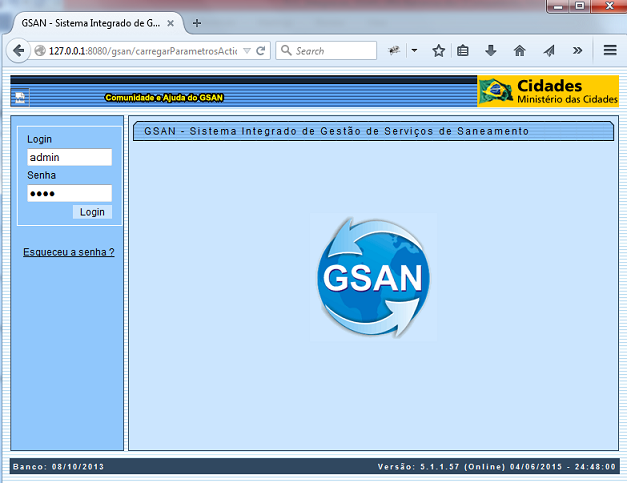
\includegraphics{figuras/gsan_online.png}	
	\legend {\fontsize{10}{12}\selectfont {Fonte: Autoria Própria}.}
\end{figure}


A credencial de acesso criada por padrão é: \\
\textbf{Login}: admin \\
\textbf{Senha}: gcom \\
Após inserir a credencial de acesso acima teremos acesso as todas as funcionalidades dos módulos do sistema GSAN.


\section{Asterisk}
A ferramenta de código aberto Asterisk desenvolvida pela Digium, disponibiliza as principais funcionalidades que um \textit{Call Center} necessita, dentre elas a criação de Ramais, Troncos, Rotas, configuração Plano de Discagens, Gravação de Voz, Conferência, Filas, Unidade de Resposta Audível entre diversos outros recursos que podem ser explorados e utilizados, podendo ser utilizado como um PABX IP, assim como se integrado a soluções VoIP ou a rede de telefonia publica.
Com tantos recursos disponíveis e sendo multiplataforma a ferramenta Asterisk está muito bem preparada para atender as expectativas, principalmente pelo fato de disponibilizar protocolos de comunicação com sistemas externos, por exemplo, o protocolo AGI (\textit{Asterisk Gateway Interface}), permite o consumo de recursos externos ao Asterisk, já o protocolo AMI (\textit{Asterisk Manager Interface}) permite que aplicações externas enviem ordens para serem executadas no Asterisk, dessa forma a solução pode ser muito bem integrada a sistemas legados.


\subsection{Asterisk Conceitos}

A ferramenta tem como base o Plano de Discagem, sendo ele responsável em definir o que deve acontecer, seja no momento em que for recepcionada uma ligação ou quando for digitado algum número. No plano de discagem podemos definir separações lógicas denominadas contextos, responsáveis em definir um comportamento utilizando os recursos nativos para determinar as instruções (extensões), por exemplo, podemos criar um contexto para definir o que deve acontecer ao receber ligações da rede pública e outro para definir o comportamento para as ligações advindas de ramais internos:

\begin{flushleft}

\textbf{[PSTN]} \\
\textit{exten => 2000,1,Answer();} \\
Contexto chamado “PSTN”, utiliza a extensão 2000, com prioridade 1 e aplicação Answer.\\

\textbf{[RAMAIS\_INTERNOS]} \\
exten => 2001,1, Playback(AVISO\_GERAL); \\
Contexto chamado “RAMAIS\_INTERNOS”, utiliza a extensão 2001, com prioridade 1 e aplicação Playback para tocar o áudio AVISO\_GERAL.\\
\end{flushleft}

O número 2000 no contexto “PSTN” utilizando na extensão representa o número informado pelo Originador da chamada, a prioridade trata-se de um parâmetro que representa a ordem de execução das aplicações, normalmente descritos de forma sequencial, já as aplicações são utilizadas para realizar uma ação qualquer. Em cada extensão (exten), podemos utilizar recursos de aplicativos nativos da ferramenta, sejam eles para atender, desligar, gravar o áudio entre outros recursos, dessa forma podemos definir o comportamento para o contexto, assim como realizar a transferência para outros contextos.


\subsection{Asterisk Instalação}

A instalação do Asterisk muita das vezes é uma tarefa cansativa e exige bastante atenção, pois a configuração deve ser realizada em arquivos de texto em uma sintaxe estabelecida pela ferramenta, atualmente existem diversas soluções que fornecem uma interface gráfica para tornar esse processo mais intuitivo e prático, neste trabalho foi utilizada uma distribuição chamada Disc-OS na versão 2.0, que disponibiliza uma interface web para realizar a configuração do Asterisk 1.4, para realizar o processo de instalação do Disc-OS, foram seguidos os passos descritos por Jilsimaico Darú (DARÚ, 2008), após a realização dos procedimentos, ao iniciar a distribuição Disc-OS automaticamente será iniciado o serviço do Asterisk, dessa forma para acessar o sistema basta digitar no navegador o endereço IP do terminal que está executando o sistema, visualizando a página conforme a figura 8 abaixo:


%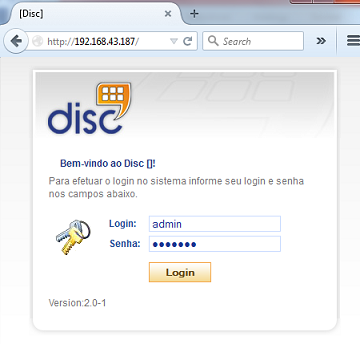
\includegraphics[scale=1]{figuras/pagina_inicial_asterisk}
\begin{center}
	IMAGEM PENDENTE \\
	Figura 8: Acessando página inicial da Interface WEB do Disc-OS \\
	Fonte: Autoria Própria \\
\end{center}

Para acessar as funcionalidades do sistema basta inserir a seguinte credencial de acesso:\\
\textbf{Login}: admin\\
\textbf{Senha}: disc-os\\


% REVISAO BIBLIOGRAFICA
\chapter[Revisão Bibliográfica]{\textbf{R}evisão \textbf{B}ibliográfica}
%\addcontentsline{toc}{chapter}{Revisão Bibliográfica}

\textit{Neste capítulo será apresentado o conceito dos \textit{frameworks} utilizados neste trabalho, além de justificar o motivo que levou a ser utilizados e destacar vantagens obtidas em seu uso.}


\section{Tecnologias Utilizadas}

No estudo para propor uma solução viável e consistente de integração entre sistemas, que seja realmente eficiente, é necessário entender todo o contexto em que está sendo operado o Sistema de Informação GSAN, visando identificar as informações mais relevantes acessadas pelo atendimento ao cliente, as principais dificuldades enfrentadas e os desafios que norteiam esse módulo do sistema. 


\subsection{GSAN - Detalhamento Técnico }

O GSAN por ser um sistema de informação adaptável a empresas de pequeno, médio e grande porte, contemplando soluções dos mais diversos requisitos, entre eles Cadastramento, Micromedição, Faturamento, Arrecadação, Cobrança, Negativação e Atendimento ao Cliente. Fornecendo de forma razoavelmente flexível as configurações e detalhes operacionais das rotinas, disponível em ambiente Web utilizando recursos de tecnologias software livre.

Para realização de melhorias no sistema GSAN faz-se necessário o ter conhecimento sobre os principais frameworks utilizados, a linguagem de programação utilizada e alguns conceitos de Saneamento que serão abordados.
Dos principais \textit{frameworks} utilizados, destaco o uso dos seguintes: \\

\textbf{Hibernate\footnote{Disponível em \url{http://www.hibernate.org}}}: Trata-se de um robusto framework de persistência de objetos relacionais, que fornece facilmente meios para realizar o mapeamento das entidades do sistema e diminui a complexidade de acesso a base de dados.\\

\textbf{Apache Struts\footnote{Disponível em \url{http://struts.apache.org/}}}: Tem como característica principal a sua utilização na construção de controladores utilizando o padrão \textit{Model View Control} (MVC) que se trata da separação das camadas utilizadas em uma aplicação, fornecendo uma maior organização no código fonte e contribui para futuras manutenções \cite{fowler2003}. 

O sistema GSAN faz uso da plataforma Java, lançado na versão Java Develop Kit (JDK) 1.5, utilizando recursos especificados pela \textit{Java Enterprise Edition} (JEE) \cite{PORTAL:2014}, essencialmente o container \textit{Enterprise Java Bean} (EJB), \textit{Java Server Pages }(JSP) e \textit{Servlets} que são executadas dentro de um servidor de aplicação Java EE.


\subsection{Asterisk - Detalhamento Técnico}
A ferramenta de código aberto Asterisk\footnote{Disponível em \url{http://www.asterisk.org}}, tem algumas características importantes e fundamentais para o estudo além de ser uma implementação de uma central telefônica que permite que clientes se comuniquem, tem outros recursos interessantes que fazem da ferramenta uma peça chave no processo da integração proposta, recursos como respostas interativas, correios de voz, realização de conferencias, distribuição automática de chamadas, além de ser flexível a adição de novos recursos tanto por meio de scripts na própria linguagem do Asterisk como também por meio de códigos em linguagem C entre outras formas de customização da ferramenta. Desenvolvido pela empresa Digium sob licença GPL (\textit{General Public Lisence}), atualmente portável em versões Linux, Windows e Mac OS, suportando protocolos de Voz sobre IP (VoIP), assim como SIP e H.323 entre outros. O próprio Asterisk contém um protocolo próprio chamado IAX fornecendo um melhor desempenho entre os entroncamentos entre os servidores Asterisk para casos de maior complexidade.

\subsection{Simple Object Access Protocol}
O protocolo SOAP\footnote{Disponível em  \url{http://www.w3.org/TR/soap}} (Simple Object Access Protocol) tem o objetivo de possibilitar a troca de informações estruturadas em Linguagem de Marcação Extensível (XML), para sistemas distribuídos. A negociação e transmissão de mensagens foram baseadas em outros em outros protocolos de serviços como o HTTP (Hypertext Transfer Protocol) e RPC (Remote Procedure Call), possibilitando a utilização para realizar integrações entre softwares.

\subsection{Asterisk Gateway Interface}
O software Asterisk possui uma interface de comunicação chamado AGI (\textit{Asterisk Gateway Interface}) \cite{asteriskAgi}, que tem como objetivo prover uma maior flexibilidade para adaptar soluções de linguagens diferentes, com esta interface se torna possível a comunicação com recursos externos através de requisição semelhantes ao CGI(\textit{Common Gateway Interface}) de servidores web, onde as requisições são originadas pelo próprio Asterisk, existem diversos \textit{frameworks} que implementam essa interface de comunicação, para este trabalho será utilizado o Asterisk-Java\footnote{Disponível em: \url{http://www.asterisk-java.org}}\label{key:asteriskjava}, por ser escrito em sob a plataforma Java e compatível com as tecnologias que foram utilizadas para a comunicação com o WebService do sistema GSAN.
O \textit{framework} Asterisk-Java possui diversos recursos disponíveis para comunicação com a ferramenta Asterisk, a seguir pode ser visto alguns dos principais propostos pelo framework;

\begin{itemize}
	\item Comunicação AGI - A classe BaseAgiScript.
	\item Comunicação HTTP - A classe ManagerConnection
	\item Ouvintes - As interfaces AsteriskServerListener e PropertyChangeListener.
	\item Controladores - A classes AsteriskServer e DefaultAsteriskServer
\end{itemize}


\subsection{WebServices}
O WebService\footnote{Disponível em \url{http://www.oracle.com/technetwork/java/javaee/tech/webservices-139501.html}} se trata de uma solução que permite que sistemas diferentes se comuniquem através requisições de protocolo HTTP a recursos identificados por um URI (\textit{Uniform Resource Identifier}) identifico a Web convencional, descritos e definidos usando XML (\textit{Extensible Markup Language}).

\subsection{Unidade de Resposta Audível}
A Unidade de Resposta Audível\label{key:URA} (URA) ou atendente eletrônico se trata de um software ou equipamento de \textit{Call Center}, que possibilita o atendimento das ligações de forma automática, tal solução traz como benefício à padronização dos atendimentos e tem potencial para automatização dos atendimentos, com inúmeras possibilidades de customização através de integrações com sistemas externo \cite{VIEIRA:2007}.

\subsection{Middleware}
O Middleware ou intermediário se trata de uma camada de software responsável em mediar à comunicação de outros sistemas, utilizado normalmente em ambientes que tendem a utilizar plataformas, linguagens ou protocolos de comunicação diferentes nas trocas de informação, sendo um dos recursos adotados neste trabalho, tal recurso descrito por \citeonline{ALMEIDA:2011}.

\subsection{Disc-OS}
O Disc-OS\footnote{Disponível em \url{http://sourceforge.net/projects/disc-os/}}\label{key:DISC-OS} refere-se a uma distribuição Linux (Cent-OS), customizada para utilização de PABX e PABX IP, abstrai toda a configuração de bibliotecas básicas e instalação do Asterisk (Disc-OS, 2015). Disponibiliza uma interface Web para configuração dos recursos, são algumas das vantagens, possuir disponível no idioma português brasileiro, além de tornar bem prático o processo de configurações.

\subsection{Codec}
O codec (COder/DEcoder) se trata de processo de codificação e decodificação da voz humana a ser transmitidas entre a origem e destino em meio digital \cite{VIEIRA:2007}.

\subsection{JUnit Framework}
O JUnit framework\footnote{Disponível em \url{http://junit.org/}} destina-se a garantia da qualidade do software, viabilizando a construção dos mais diversos tipos de testes através 
do seu arcabouço de recursos disponíveis, por ser software livre e adotado como padrão nas principais IDE de desenvolvimento Java, ganhou grande popularidade nas comunidades de desenvolvedores. O desenvolvimento de testes unitários tem sido adotado como métricas de qualidade na entrega do produto de software.
O \textit{framework} tornou a escrita de testes um processo fácil e intuitivo, fazendo uso de recurso da plataforma Java chamado \textit{Annotation}\label{key:annotation}, trouxe a possibilidade de padronizar os métodos de testes apenas adicionando anotações sobres os mesmo, segue abaixo algumas anotações comumente utilizadas;

\begin{itemize}
	\item @Test - Anotação que representa um método de teste.
	\item @Before - Anotação indica que o método anotado será executado sempre antes de um método de teste.
 	\item @After - Anotação indica que o método anotado será executado sempre após a um método de teste.
\end{itemize}

O JUnit possui um objeto chamado \textit{Assert}, que contém uma série de validações possíveis para checagem do resultado esperado pelo teste.


% INTEGRA��O
\chapter[Processo de Integração]{\textbf{P}rocesso de \textbf{I}ntegração}
\addcontentsline{toc}{chapter}{Processo de Integração}

\textit{Neste capítulo são apresentados os procedimentos para a integração dos sistemas envolvidos, expondo o detalhes de implementação e configuração da solução proposta.}


\section{Definição da Solução}

Após o estudo aprofundado sobre o sistema GSAN e software Asterisk foram identificadas diversas formas de realizar a integração, entre os sistemas pelo fato da existência de várias protocolos possíveis de comunicação , no entanto a solução adotada será visando a reusabilidade, baixo custo de manutenção e o uso de tecnologias que já tenham uma maturidade no mercado. Foram escolhidos os protocolos SOAP e AGI para serem implementados por um \textit{Middleware}, este será responsável em assumir o papel de intermediário entre os sistemas GSAN e Asterisk. Com o intuito de facilitar o entendimento da comunicação entre os sistemas, a seguir será exposto o diagrama de implantação da solução (figura 9) descrita acima, explanado os principais detalhes adotados nesta integração:

\begin{figure}[!htb]
	\centering
	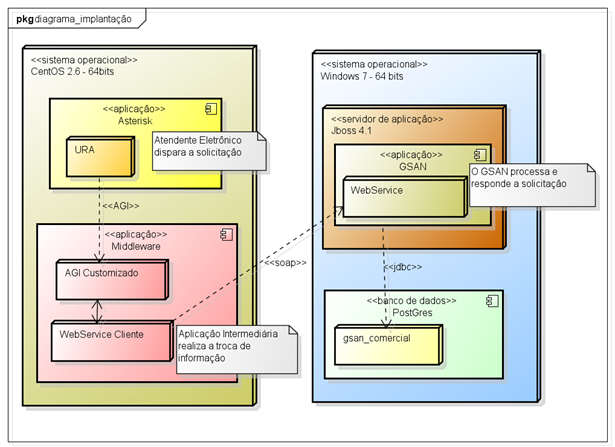
\includegraphics{figuras/diagrama_implantacao.png}
	\caption{Diagrama de implantação da solução}	
	Fonte - Autoria Própria
\end{figure}


Conforme ilustrado acima, o sistema GSAN irá prover uma interface de serviços na forma de WebServices utilizando o protocolo de comunicação SOAP (\textit{Simple Object Access Protocol}), tais serviços serão consumidos através do \textit{Middleware} intermediário denominado integrador que além de consumir os serviços do sistema GSAN, deverá também prover uma interface de serviços na forma utilizando o protocolo AGI, para então ser consumidos pelo Asterisk e responder a solicitação da Unidade de Resposta Audível.


\section{Tecnologias Utilizadas}
O processo de integração será composto por tecnologias com paradigmas diferenciados, no entanto para melhorar o entendimento dos detalhes de compatibilidades adotados segue abaixo a tabela 3 das tecnologias utilizadas e versões correspondentes.


\begin{table}[htb]
	\center
	\footnotesize
	\begin{tabular}{|p{4cm}|p{7cm}|p{2cm}|}
		\hline
		\textbf{Software} & \textbf{Finalidade} & \textbf{Versão} \\
		\hline
		Java Platform, \textit{Enterprise Edition} 5 (JEE) & Conjunto de Tecnologias e Serviços para implementar soluções da Plataforma Java com estabilidade, segurança e escalabilidade. & 5 \\
		\hline
		JBoss & Servidor de aplicação que implementa especificações JEE. & 4.0.1 sp1 \\
		\hline
		Hibernate & Framework utilizado para fazer o mapeamento objeto-relacional. É responsável pela camada de persistência. & 3.1 \\
		\hline
		PostgreSQL & Banco de dados relacional. & 9.3.4 \\
		\hline
		Apache Ant & Geração de \textit{Enterprise Application Resources} (EAR) deploy’s. & 1.6.2 \\
		\hline
		JasperReports & Tecnologia utilizada para criação de relatórios em PDF, HTML, XLS, CSV e XM.L & 1.2.2 \\
		\hline
		Struts & Framework para controle de navegação e validação Web. & 1.1	 \\
		\hline
		Disc-OS & Distribuição CentOS 2.6 que implementa interface web para a ferramenta Asterisk. & 2.0-1 \\
		\hline
		Asterisk & Software livre que permite a criação de PABX com diversos recursos. & 1.4 \\		
		\hline
		Asterisk-Java & Framework para comunicação com o Asterisk via protocolo AGI. & 1.0 \\				
	\end{tabular}
\end{table}

\begin{center}
	Tabela 3: Tecnologias utilizadas 
	Fonte: Autoria Própria
\end{center}


\section{Etapas da Integração}
O processo de integração entre os sistemas será composto por três etapas principais, das quais serão necessários para compor a solução escolhida, conforme definido abaixo e descrito nas sessões seguintes:

\begin{itemize}
	\item Implementar WebServices no Sistema GSAN 
	\item Desenvolver Middleware
	\item Customizar o Asterisk	
\end{itemize}



\chapter[Considerações sobre os Elementos Textuais]{Considerações sobre os 
Elementos Textuais}

\section{Introdução}

A regra mais rígida com respeito a Introdução é que a mesma, que é 
necessariamente parte integrante do texto, não deverá fazer agradecimentos 
a pessoas ou instituições nem comentários pessoais do autor atinentes à 
escolha ou à relevância do tema.

A Introdução obedece a critérios do Método Cientifico e a exigências 
didáticas. Na Introdução o leitor deve ser colocado dentro do espírito do 
trabalho.

Cabe mencionar que a Introdução de um trabalho pode, pelo menos em parte, 
ser escrita com grande vantagem uma vez concluído o trabalho (ou o 
Desenvolvimento e as Conclusões terem sido redigidos). Não só a pesquisa 
costuma modificar-se durante a execução, mas também, ao fim do trabalho, o 
autor tem melhor perspectiva ou visão de conjunto.

Por seu caráter didático, a Introdução deve, ao seu primeiro parágrafo, 
sugerir o mais claramente possível o que pretende o autor. Em seguida deve 
procurar situar o problema a ser examinado em relação ao desenvolvimento 
científico e técnico do momento. Assim sendo, sempre que pertinente, os 
seguintes pontos devem ser abordados: 

\begin{itemize}

	\item Contextualização ou apresentação do tema em linhas gerais de 
	forma clara e objetiva;
	\item Apresentação da justificativa e/ou relevância do tema escolhido;
	\item Apresentação da questão ou problema de pesquisa;
	\item Declaração dos objetivos, gerais e específicos do trabalho;
	\item Apresentação resumida da metodologia, e
	\item Indicação de como o trabalho estará organizado.

\end{itemize}

\section{Desenvolvimento}

O Desenvolvimento (Miolo ou Corpo do Trabalho) é subdividido em seções de 
acordo com o planejamento do autor. As seções primárias são aquelas que 
resultam da primeira divisão do texto do documento, geralmente 
correspondendo a divisão em capítulos. Seções secundárias, terciárias, 
etc., são aquelas que resultam da divisão do texto de uma seção primária, 
secundária, terciária, etc., respectivamente.

As seções primárias são numeradas consecutivamente, seguindo a série 
natural de números inteiros, a partir de 1, pela ordem de sua sucessão no 
documento.

O Desenvolvimento é a seção mais importante do trabalho, por isso exigi-se 
organização, objetividade e clareza. É conveniente dividi-lo em pelo menos 
três partes:

\begin{itemize}

	\item Referencial teórico, que corresponde a uma análise dos trabalhos 
	relevantes, encontrados na pesquisa bibliográfica sobre o assunto. 
	\item Metodologia, que é a descrição de todos os passos metodológicos 
	utilizados no trabalho. Sugere-se que se enfatize especialmente em (1) 
	População ou Sujeitos da pesquisa, (2) Materiais e equipamentos 
	utilizados e (3) Procedimentos de coleta de dados.
	\item Resultados, Discussão dos resultados e Conclusões, que é onde se 
	apresenta os dados encontrados a análise feita pelo autor à luz do 
	Referencial teórico e as Conclusões.

\end{itemize}

\section{Uso de editores de texto}

O uso de programas de edição eletrônica de textos é de livre escolha do autor. 


\part{Texto e Pós Texto}

\chapter[Elementos do Texto]{Elementos do Texto}

\section{Corpo do Texto}

O estilo de redação deve atentar a boa prática da linguagem técnica. Para a 
terminologia metrological usar o Vocabulário Internacional de Termos 
Fundamentais e Gerais de Metrologia\cite{inmetro2003}  (Instituto Nacional de Metrologia, 
2003).

Grandezas dimensionais devem ser apresentadas em unidades consistentes com 
o Sistema Internacional de Unidades  (SI). Outras unidades podem ser usadas 
como unidades secundárias entre parenteses se necessário. Exceções são 
relacionadas a unidades não-SI usadas como identificadores comerciais como 
pro exemplo \lq\lq disquete de  3$\nicefrac{1}{2}$ polegadas\rq\rq. 

Na apresentação de números ao longo do texto usar virgula para separar a 
parte decimal de um número. Resultados experimentais devem ser apresentados 
com sua respectiva incerteza de medição.

\section{Títulos de capítulos e seções}

Recomendações de formatação de seções 

\begin{description}

	\item \textbf{1 SEÇÃO PRIMÁRIA - MAIÚSCULAS; NEGRITO; TAMANHO 12;}

	\item 1.1 SEÇÃO SECUNDÁRIA – MAIÚSCULAS; NORMAL; TAMANHO 12; 

	\item \textbf{1.1.1 Seção terciária - Minúsculas, com exceção da 
	primeira letra; negrito; tamanho 12;}

	\item 1.1.1.1 Seção quaternária - Minúsculas, com exceção da primeira 
	letra; normal tamanho 12; 

 	\item \textit{1.1.1.1.1 Seção quinária - Minúsculas, com exceção da 
	primeira letra; itálico; tamanho 12.}

\end{description}

\section{Notas de rodapé}

Notas eventualmente necessárias devem ser numeradas de forma seqüencial ao 
longo do texto no formato 1, 2, 3... sendo posicionadas no rodapé de cada 
página na qual a nota é utilizada.\footnote{Como, por exemplo, esta nota}

\section{Equações}

Equações matemáticas devem ser numeradas seqüencialmente e alinhadas a 
esquerda com recuo de 0,6 cm. Usar numerais arábicos entre parênteses, 
alinhado a direita, no formato Times New Roman de 9 pts. para numerara as 
equações como mostrado na Eq. (\ref{eqn01}).

Referências a equações no corpo do texto devem ser feitas como \lq\lq Eq. 
(\ref{eqn01})\rq\rq\ quando no meio de uma frase ou como \lq\lq Equação 
(\ref{eqn01})\rq\rq\ quando no inicio de uma sentença. Um espaçamento de 11 
pontos deve ser deixado acima, abaixo e entre equações subseqüentes. Para uma 
apresentação compacta das equações deve-se usar os símbolos e expressões 
matemáticos mais adequados e parênteses para evitar ambigüidades em 
denominadores. Os símbolos usados nas equações citados no texto devem 
apresentar exatamente a mesma formatação usada nas equações.
\begin{equation}
\label{eqn01}
	\frac{d\mathbf{C}}{dw} = \frac{du}{dw}\cdot \mathbf{F}_u + 
		\frac{dv}{dw}\cdot \mathbf{F}_v 
\end{equation}

O significado de todos os símbolos mostrados nas equações deve ser apresentado 
na lista de símbolos no inicio do trabalho, embora, em certas circunstancias o 
autor possa para maior clareza descrever o significado de certos símbolos no 
corpo do texto, logo após a equação.

\section{Figuras e Gráficos}

As figuras devem ser centradas entre margens e identificadas por uma legenda 
alinhada a esquerda com recuo especial de deslocamento de 1,8 cm, com mostrado 
na Fig. (\ref{fig01}). O tamanho das fontes empregadas nos rótulos e anotações 
usadas nas figuras deve ser compatível com o usado no corpo do texto. Rótulos e 
anotações devem estar em português, com todas as grandezas mostradas em 
unidades do SI (Sistema Internacional de unidades).

Todas as figuras, gráficos e fotografias devem ser numeradas e referidas no 
corpo do texto adotando uma numeração seqüencial de identificação. As figuras e 
gráficos devem ser claras e com qualidade adequada para eventual reprodução 
posterior tanto em cores quanto em preto-e-branco.

As abscissas e ordenadas de todos os gráficos devem ser rotuladas com seus 
respectivos títulos em português seguida da unidade no SI que caracteriza a 
grandes entre colchetes. 

A referência explícita no texto à uma figura deve ser feita como 
\lq\lq Fig. (\ref{fig01})\rq\rq\ quando no meio de uma frase ou como 
\lq\lq Figura (\ref{fig01})\rq\rq\ quando no início da mesma. Referencias 
implícitas a uma dada figura devem ser feitas entre parênteses como 
(Fig. \ref{fig01}). Para referências a mais de uma figura as mesmas regras 
devem ser aplicadas usando-se o plural adequadamente. Exemplos:

\begin{itemize}
	\item \lq\lq Após os ensaios experimentais, foram obtidos os resultados 
	mostrados na Fig. (\ref{fig01}), que ...\rq\rq
	\item \lq\lq A Figura (\ref{fig01}) apresenta os resultados obtidos, onde 
	pode-se observar que ...\rq\rq
	\item \lq\lq As Figuras (1) a (3) apresentam os resultados obtidos, 
	...\rq\rq
	\item \lq\lq Verificou-se uma forte dependência entre as variáveis citadas 
	(Fig. \ref{fig01}), comprovando ...\rq\rq
\end{itemize}

Cada figura deve ser posicionada o mais próxima possível da primeira citação 
feita à mesma no texto, imediatamente após o parágrafo no qual é feita tal 
citação, se possível, na mesma página.
\begin{figure}[h]
	\centering
	\label{fig01}
		\ includegraphics[keepaspectratio=true,scale=0.3]{figuras/fig01.eps}
	\caption{Wavelets correlation coefficients}
\end{figure}

\section{Tabela}

As tabelas devem estar centradas entre margens e identificadas por uma legenda 
alinhada a esquerda, com recuo especial de deslocamento de 1,8 cm, posicionada 
acima da tabela com mostrado nas Tabs. (\ref{tab01}) e (2), a título de 
exemplo. O tamanho das fontes empregadas nos rótulos e anotações usadas nas 
tabelas deve ser compatível com o usado no corpo do texto. Rótulos e anotações 
devem estar em português. Um espaçamento de 11 pts deve ser deixado entre a 
legenda e a tabela, bem como após a tabela. 

As grandezas dimensionais mostradas em cada tabela devem apresentar unidades 
consistentes com o SI. As unidades de cada variável devem ser mostradas apenas 
na primeira linha e/ou coluna da tabela, entre colchetes 

A referência explícita no texto à uma dada tabela deve ser feita como 
\lq\lq Tab. (\ref{tab01})\rq\rq\ quando no meio de uma frase ou como 
\lq\lq Tabela (\ref{tab01})\rq\rq\ quando no início da mesma. Referências 
implícitas a uma dada tabela devem ser feitas entre parênteses como 
\lq\lq (Tab. \ref{tab01}). Para referências a mais de uma tabela as mesmas 
regras devem ser aplicadas usando-se o plural adequadamente. Exemplos:
\begin{itemize}
	\item \lq\lq Após os ensaios experimentais, foram obtidos os resultados 
	mostrados na Tab. (\ref{tab01}), que ...\rq\rq
	\item \lq\lq A Tabela (\ref{tab01}) apresenta os resultados obtidos, onde 
	pode-se observar que ...\rq\rq
	\item As Tabelas (1) a (3) apresentam os resultados obtidos, ...\rq\rq
	\item Verificou-se uma forte dependência entre as variáveis citadas 
	(Tab. \ref{tab01}), comprovando ...\rq\rq
\end{itemize}

Cada tabela deve ser posicionada o mais próxima possível da primeira citação 
feita à mesma no texto, imediatamente após o parágrafo no qual é feita a 
citação, se possível, na mesma página.

\begin{table}[h]
	\centering
	\label{tab01}
	
	\begin{tabular}{ccc}
		\toprule
		\textbf{Processing type} & \textbf{Property 1} (\%) & 
		\textbf{Property 2} $[\mu m]$ \\
		\midrule
		Process 1 & 40.0 & 22.7 \\
		Process 2 & 48.4 & 13.9 \\
		Process 3 & 39.0 & 22.5 \\
		Process 4 & 45.3 & 28.5 \\
		\bottomrule
	\end{tabular}

	\caption{Propriedades obtidades após processamento}
\end{table}

\section{Citação de Referências}

Referencias a outros trabalhos tais como artigos, teses, relatórios, etc. devem 
ser feitas no corpo do texto devem estar de acordo com a norma corrente ABNT 
NBR 6023:2002 (ABNT, 2000), esta ultima baseada nas normas ISO 690:1987:
\begin{itemize}
	\item \lq\lq \cite{bordalo1989}, mostraram que...\rq\rq

	\item \lq\lq Resultados disponíveis em \cite{coimbra1978}, \cite{clark1986} 
	e \cite{sparrow1980}, mostram que...\rq\rq
\end{itemize}

Para referências a trabalhos com até dois autores, deve-se citar o nome de 
ambos os autores, por exemplo: \lq\lq \cite{soviero1997}, mostraram 
que...\rq\rq


\chapter[Elementos do Pós-Texto]{Elementos do Pós-Texto}

Este capitulo apresenta instruções gerais sobre a elaboração e formatação dos 
elementos do pós-texto a serem apresentados em relatórios de Projeto de 
Graduação. São abordados aspectos relacionados a redação de referências 
bibliográficas, bibliografia, anexos e contra-capa.

\section{Referências Bibliográficas}

O primeiro elemento do pós-texto, inserido numa nova página, logo após o último 
capítulo do trabalho, consiste da lista das referencias bibliográficas citadas 
ao longo do texto.

Cada referência na lista deve ser justificada entre margens e redigida no 
formato Times New Roman com 11pts. Não é necessário introduzir uma linha em 
branco entre referências sucessivas.

A primeira linha de cada referencia deve ser alinhada a esquerda, com as demais 
linhas da referencia deslocadas de 0,5 cm a partir da margem esquerda. 

Todas as referências aparecendo na lista da seção \lq\lq Referências 
Bibliográficas\rq\rq\ devem estar citadas no texto. Da mesma forma o autor deve 
verificar que não há no corpo do texto citação a referências que por 
esquecimento não forma incluídas nesta seção.

As referências devem ser listadas em ordem alfabética, de acordo com o último 
nome do primeiro autor. Alguns exemplos de listagem de referencias são 
apresentados no Anexo I.

Artigos que ainda não tenham sido publicados, mesmo que tenham sido submetidos 
para publicação, não deverão ser citados. Artigos ainda não publicados mas que 
já tenham sido aceitos para publicação devem ser citados como \lq\lq in 
press\rq\rq.

A norma \cite{NBR6034:2000}, que regulamenta toda a formatação a ser usada na 
elaboração de referências a diferente tipos de fontes de consulta, deve ser 
rigidamente observada. Sugere-se a consulta do trabalho realizado por 
\cite{arruda2007}, disponível na internet.

\section{Anexos}

As informações citadas ao longo do texto como \lq\lq Anexos\rq\rq\ devem ser 
apresentadas numa seção isolada ao término do trabalho, após a seção de 
referências bibliográficas. Os anexos devem ser numerados seqüencialmente em 
algarismos romanos maiúsculos (I, II, III, ...). A primeira página dos anexos 
deve apresentar um índice conforme modelo apresentado no Anexo I, descrevendo 
cada anexo e a página inicial do mesmo.

A referência explícita no texto à um dado anexo deve ser feita como 
\lq\lq Anexo 1\rq\rq. Referências implícitas a um dado anexo devem ser feitas 
entre parênteses como (Anexo I). Para referências a mais de um anexo as mesmas 
regras devem ser aplicadas usando-se o plural adequadamente. Exemplos:
\begin{itemize}
	\item \lq\lq Os resultados detalhados dos ensaios experimentais são 
	apresentados no Anexo IV, onde ...\rq\rq

	\item \lq\lq O Anexo I apresenta os resultados obtidos, onde pode-se 
	observar que ...\rq\rq

	\item \lq\lq Os Anexos I a IV apresentam os resultados obtidos ...\rq\rq

	\item \lq\lq Verificou-se uma forte dependência entre as variáveis citadas 
	(Anexo V), comprovando ...\rq\rq
\end{itemize}



\bookmarksetup{startatroot} 

\postextual

\bibliography{bibliografia} 
\begin{apendicesenv}
	
	\partapendices

\chapter{Processo de configuração da JDK na IDE de desenvolvimento}

O sistema GSAN roda sob a JDK (\textit{Java Develop Kit}) 5, disponível atualmente no site da Oracle Coportarion, sendo necessário configurar a IDE com a versão correta para compilar o projeto, podemos configurar facilmente acessando a opção no menu superior \textit{Window > Preferences > Java > Installed JREs} em seguida será preciso adicionar uma nova JVM (\textit{Java Virtual Machine}) selecionando a opção Add e selecionar a opção Standard VM, conforme visto na figura \ref{figura:anexo1};

\begin{figure}[H]
	\centering
	\caption*{\textbf{Selecionar Tipo de JVM.}}
	\label{figura:anexo1}
	\begin{subfigure}[H]{\textwidth}
		\centering
		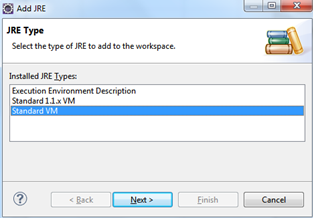
\includegraphics{figuras/anexo/selectJVM.png}
		\legend {\fontsize{10}{12}\selectfont {Fonte: Autoria Própria}.}	
	\end{subfigure}
\end{figure}


Após a seleção é preciso confirmar a ação clicando em Next, na nova janela exibida o botão Directory... permite localizar o diretório onde está a versão do JDK que será utilizada, dessa forma deve ser selecionado o diretório raiz da versão, no exemplo representado por \textit{C:/pessoal/java/jdk1.5.0\_22}, conforme visto na figura \ref{figura:anexo2};

\begin{figure}[H]
	\centering
	\caption*{\textbf{Adicionar nova JRE na IDE.}}
	\label{figura:anexo2}
	\begin{subfigure}[H]{\textwidth}
		\centering
		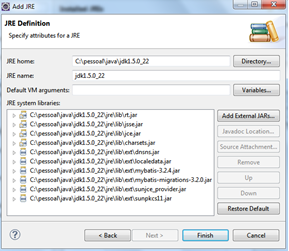
\includegraphics{figuras/anexo/addJRE.png}
		\legend {\fontsize{10}{12}\selectfont {Fonte: Autoria Própria}.}	
	\end{subfigure}
\end{figure}

A própria IDE já preenche o JRE name, caso isso não ocorra será necessário preencher este campo de preferência com o nome da versão do JDK utilizada, realizado este passo a IDE terá condições de compilar as instruções contidas no fonte.  Com isso será necessário importa o projeto no GSAN na IDE de desenvolvimento, selecionando a opção \textit{File > Import..}, abrirá um janela onde deve ser selecionando a opção \textit{General > Existing Projects into Workspace}, em seguida através do botão \textit{Browser} será possível localizar o diretório onde está o fonte do sistema GSAN, conforme ilustrado na figura \ref{figura:anexo3};

\begin{figure}[H]
	\centering
	\caption*{\textbf{Importar Sistema GSAN na IDE.}}
	\label{figura:anexo3}
	\begin{subfigure}[H]{\textwidth}
		\centering
		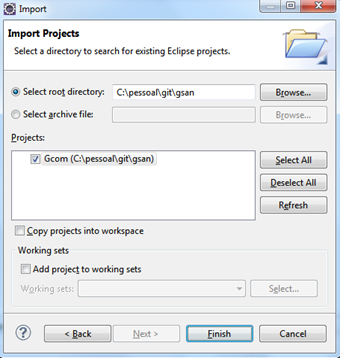
\includegraphics{figuras/anexo/importGSAN.png}
		\legend {\fontsize{10}{12}\selectfont {Fonte: Autoria Própria}.}	
	\end{subfigure}
\end{figure}


Feito isso precisa somente pressionar o botão de \textit{Finish}, para confirmar a importação do projeto para a IDE de desenvolvimento.

\chapter{Configurar variável de ambiente do servidor de aplicação Jboss}

Neste trabalho foi utilizado o projeto \textit{Open Source Jboss Community} na versão 4.0.1, compatível com as tecnologias utilizadas no GSAN, para utilizá-lo será preciso declarar uma variável de ambiente no sistema operacional, por padrão nomeado de JBOSS\_HOME contendo a localização do diretório do servidor de aplicação, no exemplo abaixo representado por \textit{C:/pessoal/jboss/jboss-4.0.1sp1}, conforme visto na figura \ref{figura:anexo4};

\begin{figure}[H]
	\centering
	\caption*{\textbf{Adicionando variável de ambiente JBOSS\_HOME.}}
	\label{figura:anexo4}
	\begin{subfigure}[H]{\textwidth}
		\centering
		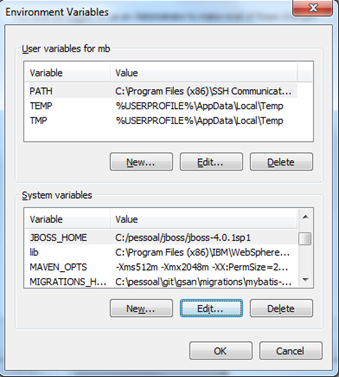
\includegraphics{figuras/anexo/var_JBOSS_HOME.png}
		\legend {\fontsize{10}{12}\selectfont {Fonte: Autoria Própria}.}	
	\end{subfigure}
\end{figure}


Após a criação desta variável de ambiente, será preciso atualizar a variável de ambiente chamada PATH que reúne as variáveis utilizadas no sistema operacional, adicionando ao final o seguinte texto \textit{\%JBOSS\_HOME\%/bin;} para que o sistema operacional consiga localizar o diretório /bin do servidor de aplicação que contém o script de inicialização do servidor chamado \textit{run.bat} para sistemas Windows e \textit{run.sh} para sistemas Unix, neste script é possível modificar os parâmetros utilizados na execução do servidor de aplicação sob a JVM para a alocação de memória assim como habilitar a utilização de técnicas de debug remoto das aplicações.


\chapter{Configuração do Fluxo da URA}
Segue abaixo a configuração do fluxo completo da URA, configurado no seguinte arquivo de configuração \textit{/etc/asterisk/extension.conf};
\\\\
; Declarando o contexto de boas vindas para executar o áudio ‘inicial’ \\
; o dígito representa a rotina associada abaixo: \\
; 1 – Contexto de identificação do Cliente. \\
; 2 – Falar com o atendente. \\
\textbf{[disc-ivr-BOAS\_VINDAS] }	 \\
exten => s,1,Playback(custom/inicial)  \\
exten => 1,1,Goto(disc-ivr-IDENTIFICACAO,7001,1)  \\
exten => 2,1,Goto(FALAR\_ATENDENTE,s,1)  \\
 \\
; Declarando o contexto de identificação do cliente, executa o áudio  \\
; ‘identificacao’ e redireciona para o contexto de PESQUISAR\_CLIENTE \\
; executa o áudio ‘pronto’ e ‘numero\_ra’, soletra o numero do RA e  \\
; direciona para o Menu principal. \\
\textbf{[disc-ivr-IDENTIFICACAO]} \\
exten => 7001,1,Playback(custom/identificacao) \\
exten => 7001,2,Goto(PESQUISAR\_CLIENTE,s,1) \\
exten => 7001,3,Playback(custom/pronto) \\
exten => 7001,4,Playback(custom/numero\_ra) \\
exten => 7001,5,SayDigits(\${NUMERO\_RA}) \\
exten => 7001,6,Goto(disc-ivr-MENU,7002,1) \\
 \\
; Declara o context do Menu Principal, executa o áudio ‘menu’, \\
; o dígito representa a rotina associada abaixo: \\
; 1 – Serviço de 2ª via de Conta \\
; 2 – Serviço de Informar Falta de Água \\
; 3 – Serviço de Solicitar Restabelecimento da Ligação \\
; 4 – Falar com o atendente. \\
\textbf{[disc-ivr-MENU]} \\
exten => 7002,1,Playback(custom/menu) \\
exten => 1,1,Goto(disc-ivr-2VIA,7003,1) \\
exten => 2,1,Goto(disc-ivr-INFORMAR\_FALTA\_AGUA,7004,1) \\
exten => 3,1,Goto(disc-ivr-SOLICITAR\_RESTABELECIMENTO,7005,1) \\
exten => 4,1,Goto(FALAR\_ATENDENTE,s,1) \\
 \\
; Declarando o contexto de 2ª via, executa o aúdio ‘2via’ \\
; redireciona para o contexto de obter segunda via e \\
; desliga a ligação. \\
\textbf{[disc-ivr-2VIA]} \\
exten => 7003,1,Playback(custom/2via) \\
exten => 7003,2,Goto(OBTER\_SEGUNDA\_VIA,s,1) \\
exten => 7003,3,Hangup() \\
 \\
; Declarando o contexto disc-ivr-INFORMAR\_FALTA\_AGUA \\
; Executa o áudio ‘falta\_agua\_abrir\_chamado’  \\
; Redireciona para o contexto INFORMAR\_FALTA\_AGUA \\
; Executa o áudio ‘sucesso’ \\
; Desliga a ligação \\
\textbf{[disc-ivr-INFORMAR\_FALTA\_AGUA]} \\
exten => 7004,1,Playback(custom/falta\_agua\_abrir\_chamado) \\
exten => 7004,2,Goto(INFORMAR\_FALTA\_AGUA,s,1) \\
exten => 7004,3,Playback(custom/sucesso) \\
exten => 7004,4,Hangup() \\
 \\
; Declarando o contexto disc-ivr-SOLICITAR\_RESTABELECIMENTO \\
; Executa o áudio ‘restabelecimento’  \\
; Redireciona para o contexto SOLICITAR\_RESTABELECIMENTO \\
; Executa o áudio ‘sucesso’ \\
; Desliga a ligação \\
\textbf{[disc-ivr-SOLICITAR\_RESTABELECIMENTO]} \\
exten => 7005,1,Playback(custom/restabelecimento) \\
exten => 7005,2,Goto(SOLICITAR\_RESTABELECIMENTO,s,1) \\
exten => 7005,3,Playback(custom/sucesso) \\
exten => 7005,4,Hangup() \\
 \\
; Declarando o contexto ‘PESQUISAR\_CLIENTE’ \\
; Atende a ligação \\
; Executa o áudio ‘beep’ \\
; Defini o tempo limite de espera entre a discagem dos dígitos \\
; Defini o tempo limite de espera do primeiro dígito \\
; Ler os digitos informados \\
; Cria a variável ‘CLIENTE\_IMOVEL’ recebendo os digitos. \\
; Executa uma requisição Agi para ‘192.168.43.2/pesquisar.imovel.cliente.agi’ \\
; Exibe o ID\_IMOVEL \\
; Verifica a situação da requisição realizada \\
; Caso seja ‘SUCESSO’ redireciona para o contexto disc-ivr-IDENTIFICACAO \\
; Caso seja diferente de sucesso redireciona para FALAR\_ATENDENTE \\
\textbf{[PESQUISAR\_CLIENTE]} \\
exten => s,1,Answer() \\
exten => s,n,PlayBack(beep) \\
exten => s,n,Set(TIMEOUT(digit)=3)  \\
exten => s,n,Set(TIMEOUT(response)=7)  \\
exten => s,n,Read(NUMERO) ; LER OS DIGITOS \\
exten => s,n,Set(CLIENTE\_IMOVEL=\${NUMERO}) \\
exten => s,n,Agi(agi://192.168.43.2/pesquisar.imovel.cliente.agi) \\
exten => s,n,NoOp(\${ID\_IMOVEL}) \\
exten => s,n,GotoIf(\$["\${SITUACAO}" == "SUCESSO"]?ok:falha) \\
exten => s,n(ok),Goto(disc-ivr-IDENTIFICACAO,7001,3) \\
exten => s,n(falha),Goto(FALAR\_ATENDENTE,s,1) \\
 \\
; Declarando o contexto ‘OBTER\_SEGUNDA\_VIA’ \\
; Atende a ligação \\
; Executa uma requisição Agi para ‘192.168.43.2/segunda.via.agi’ \\
; Printa o ‘ID\_IMOVEL’ \\
; Verifica a situação da requisição realizada \\
; Caso seja ‘SUCESSO’ redireciona para o contexto ‘disc-ivr-2VIA’ \\
; Caso seja diferente de sucesso redireciona para ‘FALAR\_ATENDENTE’ \\
\textbf{[OBTER\_SEGUNDA\_VIA]} \\
exten => s,1,Answer() \\
exten => s,n,Agi(agi://192.168.43.2/segunda.via.agi) \\
exten => s,n,NoOp(\${ID\_IMOVEL}) \\
exten => s,n,GotoIf(\$["\${SITUACAO}" == "SUCESSO"]?ok:falha) \\
exten => s,n(ok),Goto(disc-ivr-2VIA,7003,3) \\
exten => s,n(falha),Goto(FALAR\_ATENDENTE,s,1) \\
\\
; Declarando o contexto ‘INFORMAR\_FALTA\_AGUA’ \\
; Atende a ligação \\
; Executa uma requisição Agi para ‘192.168.43.2/falta.agua.agi’ \\
; Verifica a situação da requisição realizada \\
; Caso seja ‘SUCESSO’ redireciona para o contexto \\
; ‘disc-ivr-NFORMAR\_FALTA\_AGUA’ \\
; Caso seja diferente de sucesso redireciona para ‘FALAR\_ATENDENTE’ \\
\textbf{[INFORMAR\_FALTA\_AGUA]} \\
exten => s,1,Answer() \\
exten => s,n,Agi(agi://192.168.43.2/falta.agua.agi) \\
exten => s,n,GotoIf(\$["\${SITUACAO}" == "SUCESSO"]?ok:falha) \\
exten => s,n(ok),Goto(disc-ivr-INFORMAR\_FALTA\_AGUA,7004,3) \\
exten => s,n(falha),Goto(FALAR\_ATENDENTE,s,1) \\
 \\
; Declarando o contexto ‘SOLICITAR\_RESTABELECIMENTO’ \\
; Atende a ligação \\
; Executa uma requisição Agi para ‘192.168.43.2/restabelecimento.ligacao.agi’ \\
; Verifica a situação da requisição realizada \\
; Caso seja ‘SUCESSO’ redireciona p/ o contexto \\
; ‘disc-ivr-SOLICITAR\_RESTABELECIMENTO \\
; Caso seja diferente de sucesso redireciona para ‘FALAR\_ATENDENTE’ \\
\textbf{[SOLICITAR\_RESTABELECIMENTO]} \\
exten => s,1,Answer() \\
exten => s,n,Agi(agi://192.168.43.2/restabelecimento.ligacao.agi) \\
exten => s,n,GotoIf(\$["\${SITUACAO}" == "SUCESSO"]?ok:falha) \\
exten => s,n(ok),Goto(disc-ivr-SOLICITAR\_RESTABELECIMENTO,7005,3) \\
exten => s,n(falha),Goto(FALAR\_ATENDENTE,s,1) \\
 \\
; Declarando o contexto ‘FALAR\_ATENDENTE’ \\
; Executa o áudio ‘ligacao\_redirecionada’ \\
; Realiza uma ligação para o ‘ATENDENTE’ \\
\textbf{[FALAR\_ATENDENTE]} \\
exten => s,1,PlayBack(custom/ligacao\_redirecionada) \\
exten => s,2,Dial(SIP/ATENDENTE) \\


\chapter{Registros de Atendimentos Gerados}

A execução dos cenários de testes resultaram na criação dos seguintes Registros de Atendimentos no sistema GSAN,
a seguir pode ser consultado o detalhamento sobre os Registros de Atendimentos gerados para o serviço Informar Falta de Água.
\begin{figure}[H]
	\centering
	\caption*{\textbf{Informar Falta de Água - Cenário 1 Detalhado.}}
	\begin{subfigure}[H]{\textwidth}
		\centering
		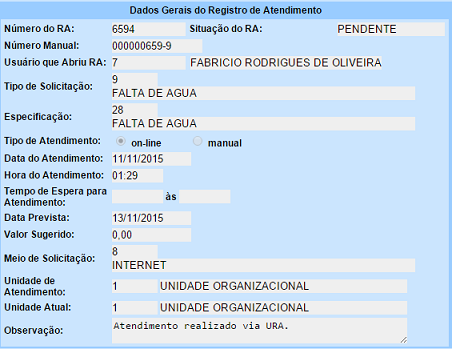
\includegraphics{figuras/anexo/falta_agua/detalhe_1.png}
		\legend {\fontsize{10}{12}\selectfont {Fonte: Autoria Própria}.}	
	\end{subfigure}
\end{figure}

\begin{figure}[H]
	\centering
	\caption*{\textbf{Informar Falta de Água - Cenário 2 Detalhado.}}
	\begin{subfigure}[H]{\textwidth}
		\centering
		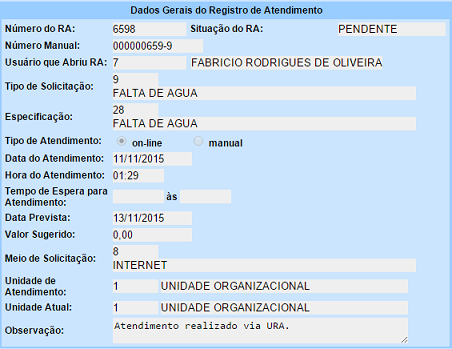
\includegraphics{figuras/anexo/falta_agua/detalhe_2.png}
		\legend {\fontsize{10}{12}\selectfont {Fonte: Autoria Própria}.}	
	\end{subfigure}
\end{figure}

\begin{figure}[H]
	\centering
	\caption*{\textbf{Informar Falta de Água - Cenário 3 Detalhado.}}
	\begin{subfigure}[H]{\textwidth}
		\centering
		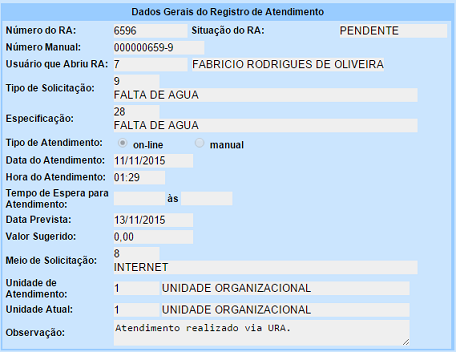
\includegraphics{figuras/anexo/falta_agua/detalhe_3.png}
		\legend {\fontsize{10}{12}\selectfont {Fonte: Autoria Própria}.}	
	\end{subfigure}
\end{figure}



A seguir pode ser consultado os registros de atendimentos abertos pela execução da suíte de testes automatizados para o serviço Solicitar Restabelecimento da Ligação de Água;

\begin{figure}[H]
	\centering
	\caption*{\textbf{Solicitar Restabelecimento da Ligação de Água - Cenário 1 Detalhado.}}
	\begin{subfigure}[H]{\textwidth}
		\centering
		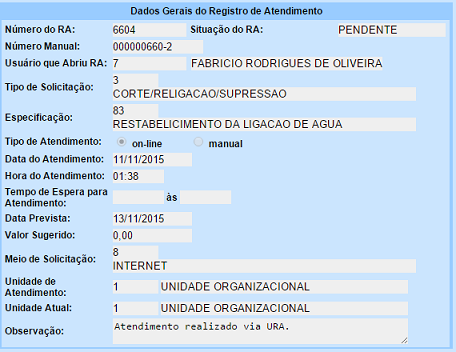
\includegraphics{figuras/anexo/restabelecer/detalhe_1.png}
		\legend {\fontsize{10}{12}\selectfont {Fonte: Autoria Própria}.}	
	\end{subfigure}
\end{figure}

\begin{figure}[H]
	\centering
	\caption*{\textbf{Solicitar Restabelecimento da Ligação de Água - Cenário 2 Detalhado.}}
	\begin{subfigure}[H]{\textwidth}
		\centering
		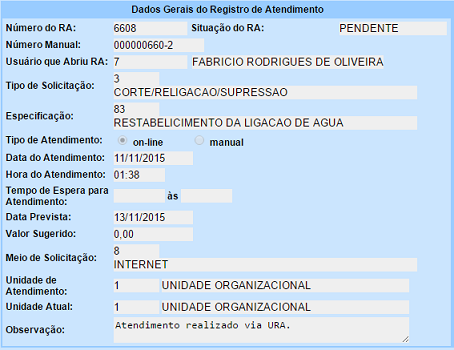
\includegraphics{figuras/anexo/restabelecer/detalhe_2.png}
		\legend {\fontsize{10}{12}\selectfont {Fonte: Autoria Própria}.}	
	\end{subfigure}
\end{figure}

\begin{figure}[H]
	\centering
	\caption*{\textbf{Solicitar Restabelecimento da Ligação de Água - Cenário 3 Detalhado.}}
	\begin{subfigure}[H]{\textwidth}
		\centering
		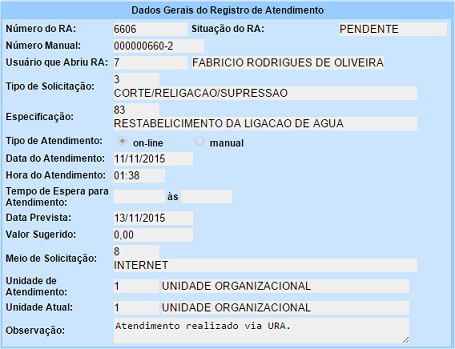
\includegraphics{figuras/anexo/restabelecer/detalhe_3.png}
		\legend {\fontsize{10}{12}\selectfont {Fonte: Autoria Própria}.}	
	\end{subfigure}
\end{figure}


\end{apendicesenv}




\begin{anexosenv}

\partanexos

\chapter{Primeiro Anexo}

Texto do primeiro anexo.

\chapter{Segundo Anexo}

Texto do segundo anexo.

\end{anexosenv}


\printindex

\end{document}

